%==================================================================================
%==================================================================================
\documentclass[11pt]{beamer}
%==================================================================================
%==================================================================================
\mode<presentation>
{
  \usetheme{default}      % or try Darmstadt, Madrid, Warsaw, ...
  \usecolortheme{default} % or try albatross, beaver, crane, ...
  \usefonttheme{default}  % or try serif, structurebold, ...
  \setbeamertemplate{navigation symbols}{}
  \setbeamertemplate{caption}[numbered]
  \setbeamertemplate{footline}[frame number]
  \setbeamerfont{frametitle}{size=\large,series=\bfseries}
  \setbeamercolor{frametitle}{fg=blue}
  \setbeamercolor{background canvas}{bg=white}
  \setbeamercolor{normal text}{fg=black}
}

%==================================================================================

% \usepackage[
% 	colorlinks=true,
% 	urlcolor=blue,
% 	linkcolor=blue
% ]{hyperref}
\usepackage[english]{babel}
\usepackage[utf8x]{inputenc}
\usepackage{graphicx}
\definecolor{snow}{rgb}{1.000,0.980,0.980}
\definecolor{snow1}{rgb}{1.000,0.980,0.980}
\definecolor{snow2}{rgb}{0.933,0.914,0.914}
\definecolor{snow3}{rgb}{0.804,0.788,0.788}
\definecolor{snow4}{rgb}{0.545,0.537,0.537}
\definecolor{GhostWhite}{rgb}{0.973,0.973,1.000}
\definecolor{WhiteSmoke}{rgb}{0.961,0.961,0.961}
\definecolor{gainsboro}{rgb}{0.863,0.863,0.863}
\definecolor{FloralWhite}{rgb}{1.000,0.980,0.941}
\definecolor{OldLace}{rgb}{0.992,0.961,0.902}
\definecolor{linen}{rgb}{0.980,0.941,0.902}
\definecolor{AntiqueWhite}{rgb}{0.980,0.922,0.843}
\definecolor{PapayaWhip}{rgb}{1.000,0.937,0.835}
\definecolor{BlanchedAlmond}{rgb}{1.000,0.922,0.804}
\definecolor{bisque}{rgb}{1.000,0.894,0.769}
\definecolor{PeachPuff}{rgb}{1.000,0.855,0.725}
\definecolor{NavajoWhite}{rgb}{1.000,0.871,0.678}
\definecolor{moccasin}{rgb}{1.000,0.894,0.710}
\definecolor{cornsilk}{rgb}{1.000,0.973,0.863}
\definecolor{ivory}{rgb}{1.000,1.000,0.941}
\definecolor{LemonChiffon}{rgb}{1.000,0.980,0.804}
\definecolor{seashell}{rgb}{1.000,0.961,0.933}
\definecolor{honeydew}{rgb}{0.941,1.000,0.941}
\definecolor{MintCream}{rgb}{0.961,1.000,0.980}
\definecolor{azure}{rgb}{0.941,1.000,1.000}
\definecolor{AliceBlue}{rgb}{0.941,0.973,1.000}
\definecolor{lavender}{rgb}{0.902,0.902,0.980}
\definecolor{LavenderBlush}{rgb}{1.000,0.941,0.961}
\definecolor{MistyRose}{rgb}{1.000,0.894,0.882}
\definecolor{white}{rgb}{1.000,1.000,1.000}
\definecolor{black}{rgb}{0.000,0.000,0.000}
\definecolor{DarkSlateGray}{rgb}{0.184,0.310,0.310}
\definecolor{DimGray}{rgb}{0.412,0.412,0.412}
\definecolor{SlateGray}{rgb}{0.439,0.502,0.565}
\definecolor{LightSlateGray}{rgb}{0.467,0.533,0.600}
\definecolor{gray}{rgb}{0.745,0.745,0.745}
\definecolor{LightGray}{rgb}{0.827,0.827,0.827}
\definecolor{MidnightBlue}{rgb}{0.098,0.098,0.439}
\definecolor{navy}{rgb}{0.000,0.000,0.502}
\definecolor{NavyBlue}{rgb}{0.000,0.000,0.502}
\definecolor{CornflowerBlue}{rgb}{0.392,0.584,0.929}
\definecolor{DarkSlateBlue}{rgb}{0.282,0.239,0.545}
\definecolor{SlateBlue}{rgb}{0.416,0.353,0.804}
\definecolor{MediumSlateBlue}{rgb}{0.482,0.408,0.933}
\definecolor{LightSlateBlue}{rgb}{0.518,0.439,1.000}
\definecolor{MediumBlue}{rgb}{0.000,0.000,0.804}
\definecolor{RoyalBlue}{rgb}{0.255,0.412,0.882}
\definecolor{blue}{rgb}{0.000,0.000,1.000}
\definecolor{DodgerBlue}{rgb}{0.118,0.565,1.000}
\definecolor{DeepSkyBlue}{rgb}{0.000,0.749,1.000}
\definecolor{SkyBlue}{rgb}{0.529,0.808,0.922}
\definecolor{LightSkyBlue}{rgb}{0.529,0.808,0.980}
\definecolor{SteelBlue}{rgb}{0.275,0.510,0.706}
\definecolor{LightSteelBlue}{rgb}{0.690,0.769,0.871}
\definecolor{LightBlue}{rgb}{0.678,0.847,0.902}
\definecolor{PowderBlue}{rgb}{0.690,0.878,0.902}
\definecolor{PaleTurquoise}{rgb}{0.686,0.933,0.933}
\definecolor{DarkTurquoise}{rgb}{0.000,0.808,0.820}
\definecolor{MediumTurquoise}{rgb}{0.282,0.820,0.800}
\definecolor{turquoise}{rgb}{0.251,0.878,0.816}
\definecolor{cyan}{rgb}{0.000,1.000,1.000}
\definecolor{LightCyan}{rgb}{0.878,1.000,1.000}
\definecolor{CadetBlue}{rgb}{0.373,0.620,0.627}
\definecolor{MediumAquamarine}{rgb}{0.400,0.804,0.667}
\definecolor{aquamarine}{rgb}{0.498,1.000,0.831}
\definecolor{DarkGreen}{rgb}{0.000,0.392,0.000}
\definecolor{DarkOliveGreen}{rgb}{0.333,0.420,0.184}
\definecolor{DarkSeaGreen}{rgb}{0.561,0.737,0.561}
\definecolor{SeaGreen}{rgb}{0.180,0.545,0.341}
\definecolor{MediumSeaGreen}{rgb}{0.235,0.702,0.443}
\definecolor{LightSeaGreen}{rgb}{0.125,0.698,0.667}
\definecolor{PaleGreen}{rgb}{0.596,0.984,0.596}
\definecolor{SpringGreen}{rgb}{0.000,1.000,0.498}
\definecolor{LawnGreen}{rgb}{0.486,0.988,0.000}
\definecolor{green}{rgb}{0.000,1.000,0.000}
\definecolor{chartreuse}{rgb}{0.498,1.000,0.000}
\definecolor{MediumSpringGreen}{rgb}{0.000,0.980,0.604}
\definecolor{GreenYellow}{rgb}{0.678,1.000,0.184}
\definecolor{LimeGreen}{rgb}{0.196,0.804,0.196}
\definecolor{YellowGreen}{rgb}{0.604,0.804,0.196}
\definecolor{ForestGreen}{rgb}{0.133,0.545,0.133}
\definecolor{OliveDrab}{rgb}{0.420,0.557,0.137}
\definecolor{DarkKhaki}{rgb}{0.741,0.718,0.420}
\definecolor{khaki}{rgb}{0.941,0.902,0.549}
\definecolor{PaleGoldenrod}{rgb}{0.933,0.910,0.667}
\definecolor{LightGoldenrodYellow}{rgb}{0.980,0.980,0.824}
\definecolor{LightYellow}{rgb}{1.000,1.000,0.878}
\definecolor{yellow}{rgb}{1.000,1.000,0.000}
\definecolor{gold}{rgb}{1.000,0.843,0.000}
\definecolor{LightGoldenrod}{rgb}{0.933,0.867,0.510}
\definecolor{goldenrod}{rgb}{0.855,0.647,0.125}
\definecolor{DarkGoldenrod}{rgb}{0.722,0.525,0.043}
\definecolor{RosyBrown}{rgb}{0.737,0.561,0.561}
\definecolor{IndianRed}{rgb}{0.804,0.361,0.361}
\definecolor{SaddleBrown}{rgb}{0.545,0.271,0.075}
\definecolor{sienna}{rgb}{0.627,0.322,0.176}
\definecolor{peru}{rgb}{0.804,0.522,0.247}
\definecolor{burlywood}{rgb}{0.871,0.722,0.529}
\definecolor{beige}{rgb}{0.961,0.961,0.863}
\definecolor{wheat}{rgb}{0.961,0.871,0.702}
\definecolor{SandyBrown}{rgb}{0.957,0.643,0.376}
\definecolor{tan}{rgb}{0.824,0.706,0.549}
\definecolor{chocolate}{rgb}{0.824,0.412,0.118}
\definecolor{firebrick}{rgb}{0.698,0.133,0.133}
\definecolor{brown}{rgb}{0.647,0.165,0.165}
\definecolor{DarkSalmon}{rgb}{0.914,0.588,0.478}
\definecolor{salmon}{rgb}{0.980,0.502,0.447}
\definecolor{LightSalmon}{rgb}{1.000,0.627,0.478}
\definecolor{orange}{rgb}{1.000,0.647,0.000}
\definecolor{DarkOrange}{rgb}{1.000,0.549,0.000}
\definecolor{coral}{rgb}{1.000,0.498,0.314}
\definecolor{LightCoral}{rgb}{0.941,0.502,0.502}
\definecolor{tomato}{rgb}{1.000,0.388,0.278}
\definecolor{OrangeRed}{rgb}{1.000,0.271,0.000}
\definecolor{red}{rgb}{1.000,0.000,0.000}
\definecolor{HotPink}{rgb}{1.000,0.412,0.706}
\definecolor{DeepPink}{rgb}{1.000,0.078,0.576}
\definecolor{pink}{rgb}{1.000,0.753,0.796}
\definecolor{LightPink}{rgb}{1.000,0.714,0.757}
\definecolor{PaleVioletRed}{rgb}{0.859,0.439,0.576}
\definecolor{maroon}{rgb}{0.690,0.188,0.376}
\definecolor{MediumVioletRed}{rgb}{0.780,0.082,0.522}
\definecolor{VioletRed}{rgb}{0.816,0.125,0.565}
\definecolor{magenta}{rgb}{1.000,0.000,1.000}
\definecolor{violet}{rgb}{0.933,0.510,0.933}
\definecolor{plum}{rgb}{0.867,0.627,0.867}
\definecolor{orchid}{rgb}{0.855,0.439,0.839}
\definecolor{MediumOrchid}{rgb}{0.729,0.333,0.827}
\definecolor{DarkOrchid}{rgb}{0.600,0.196,0.800}
\definecolor{DarkViolet}{rgb}{0.580,0.000,0.827}
\definecolor{BlueViolet}{rgb}{0.541,0.169,0.886}
\definecolor{purple}{rgb}{0.627,0.125,0.941}
\definecolor{MediumPurple}{rgb}{0.576,0.439,0.859}
\definecolor{thistle}{rgb}{0.847,0.749,0.847}
\definecolor{seashell1}{rgb}{1.000,0.961,0.933}
\definecolor{seashell2}{rgb}{0.933,0.898,0.871}
\definecolor{seashell3}{rgb}{0.804,0.773,0.749}
\definecolor{seashell4}{rgb}{0.545,0.525,0.510}
\definecolor{AntiqueWhite1}{rgb}{1.000,0.937,0.859}
\definecolor{AntiqueWhite2}{rgb}{0.933,0.875,0.800}
\definecolor{AntiqueWhite3}{rgb}{0.804,0.753,0.690}
\definecolor{AntiqueWhite4}{rgb}{0.545,0.514,0.471}
\definecolor{bisque1}{rgb}{1.000,0.894,0.769}
\definecolor{bisque2}{rgb}{0.933,0.835,0.718}
\definecolor{bisque3}{rgb}{0.804,0.718,0.620}
\definecolor{bisque4}{rgb}{0.545,0.490,0.420}
\definecolor{PeachPuff1}{rgb}{1.000,0.855,0.725}
\definecolor{PeachPuff2}{rgb}{0.933,0.796,0.678}
\definecolor{PeachPuff3}{rgb}{0.804,0.686,0.584}
\definecolor{PeachPuff4}{rgb}{0.545,0.467,0.396}
\definecolor{NavajoWhite1}{rgb}{1.000,0.871,0.678}
\definecolor{NavajoWhite2}{rgb}{0.933,0.812,0.631}
\definecolor{NavajoWhite3}{rgb}{0.804,0.702,0.545}
\definecolor{NavajoWhite4}{rgb}{0.545,0.475,0.369}
\definecolor{LemonChiffon1}{rgb}{1.000,0.980,0.804}
\definecolor{LemonChiffon2}{rgb}{0.933,0.914,0.749}
\definecolor{LemonChiffon3}{rgb}{0.804,0.788,0.647}
\definecolor{LemonChiffon4}{rgb}{0.545,0.537,0.439}
\definecolor{cornsilk1}{rgb}{1.000,0.973,0.863}
\definecolor{cornsilk2}{rgb}{0.933,0.910,0.804}
\definecolor{cornsilk3}{rgb}{0.804,0.784,0.694}
\definecolor{cornsilk4}{rgb}{0.545,0.533,0.471}
\definecolor{ivory1}{rgb}{1.000,1.000,0.941}
\definecolor{ivory2}{rgb}{0.933,0.933,0.878}
\definecolor{ivory3}{rgb}{0.804,0.804,0.757}
\definecolor{ivory4}{rgb}{0.545,0.545,0.514}
\definecolor{honeydew1}{rgb}{0.941,1.000,0.941}
\definecolor{honeydew2}{rgb}{0.878,0.933,0.878}
\definecolor{honeydew3}{rgb}{0.757,0.804,0.757}
\definecolor{honeydew4}{rgb}{0.514,0.545,0.514}
\definecolor{LavenderBlush1}{rgb}{1.000,0.941,0.961}
\definecolor{LavenderBlush2}{rgb}{0.933,0.878,0.898}
\definecolor{LavenderBlush3}{rgb}{0.804,0.757,0.773}
\definecolor{LavenderBlush4}{rgb}{0.545,0.514,0.525}
\definecolor{MistyRose1}{rgb}{1.000,0.894,0.882}
\definecolor{MistyRose2}{rgb}{0.933,0.835,0.824}
\definecolor{MistyRose3}{rgb}{0.804,0.718,0.710}
\definecolor{MistyRose4}{rgb}{0.545,0.490,0.482}
\definecolor{azure1}{rgb}{0.941,1.000,1.000}
\definecolor{azure2}{rgb}{0.878,0.933,0.933}
\definecolor{azure3}{rgb}{0.757,0.804,0.804}
\definecolor{azure4}{rgb}{0.514,0.545,0.545}
\definecolor{SlateBlue1}{rgb}{0.514,0.435,1.000}
\definecolor{SlateBlue2}{rgb}{0.478,0.404,0.933}
\definecolor{SlateBlue3}{rgb}{0.412,0.349,0.804}
\definecolor{SlateBlue4}{rgb}{0.278,0.235,0.545}
\definecolor{RoyalBlue1}{rgb}{0.282,0.463,1.000}
\definecolor{RoyalBlue2}{rgb}{0.263,0.431,0.933}
\definecolor{RoyalBlue3}{rgb}{0.227,0.373,0.804}
\definecolor{RoyalBlue4}{rgb}{0.153,0.251,0.545}
\definecolor{blue1}{rgb}{0.000,0.000,1.000}
\definecolor{blue2}{rgb}{0.000,0.000,0.933}
\definecolor{blue3}{rgb}{0.000,0.000,0.804}
\definecolor{blue4}{rgb}{0.000,0.000,0.545}
\definecolor{DodgerBlue1}{rgb}{0.118,0.565,1.000}
\definecolor{DodgerBlue2}{rgb}{0.110,0.525,0.933}
\definecolor{DodgerBlue3}{rgb}{0.094,0.455,0.804}
\definecolor{DodgerBlue4}{rgb}{0.063,0.306,0.545}
\definecolor{SteelBlue1}{rgb}{0.388,0.722,1.000}
\definecolor{SteelBlue2}{rgb}{0.361,0.675,0.933}
\definecolor{SteelBlue3}{rgb}{0.310,0.580,0.804}
\definecolor{SteelBlue4}{rgb}{0.212,0.392,0.545}
\definecolor{DeepSkyBlue1}{rgb}{0.000,0.749,1.000}
\definecolor{DeepSkyBlue2}{rgb}{0.000,0.698,0.933}
\definecolor{DeepSkyBlue3}{rgb}{0.000,0.604,0.804}
\definecolor{DeepSkyBlue4}{rgb}{0.000,0.408,0.545}
\definecolor{SkyBlue1}{rgb}{0.529,0.808,1.000}
\definecolor{SkyBlue2}{rgb}{0.494,0.753,0.933}
\definecolor{SkyBlue3}{rgb}{0.424,0.651,0.804}
\definecolor{SkyBlue4}{rgb}{0.290,0.439,0.545}
\definecolor{LightSkyBlue1}{rgb}{0.690,0.886,1.000}
\definecolor{LightSkyBlue2}{rgb}{0.643,0.827,0.933}
\definecolor{LightSkyBlue3}{rgb}{0.553,0.714,0.804}
\definecolor{LightSkyBlue4}{rgb}{0.376,0.482,0.545}
\definecolor{SlateGray1}{rgb}{0.776,0.886,1.000}
\definecolor{SlateGray2}{rgb}{0.725,0.827,0.933}
\definecolor{SlateGray3}{rgb}{0.624,0.714,0.804}
\definecolor{SlateGray4}{rgb}{0.424,0.482,0.545}
\definecolor{LightSteelBlue1}{rgb}{0.792,0.882,1.000}
\definecolor{LightSteelBlue2}{rgb}{0.737,0.824,0.933}
\definecolor{LightSteelBlue3}{rgb}{0.635,0.710,0.804}
\definecolor{LightSteelBlue4}{rgb}{0.431,0.482,0.545}
\definecolor{LightBlue1}{rgb}{0.749,0.937,1.000}
\definecolor{LightBlue2}{rgb}{0.698,0.875,0.933}
\definecolor{LightBlue3}{rgb}{0.604,0.753,0.804}
\definecolor{LightBlue4}{rgb}{0.408,0.514,0.545}
\definecolor{LightCyan1}{rgb}{0.878,1.000,1.000}
\definecolor{LightCyan2}{rgb}{0.820,0.933,0.933}
\definecolor{LightCyan3}{rgb}{0.706,0.804,0.804}
\definecolor{LightCyan4}{rgb}{0.478,0.545,0.545}
\definecolor{PaleTurquoise1}{rgb}{0.733,1.000,1.000}
\definecolor{PaleTurquoise2}{rgb}{0.682,0.933,0.933}
\definecolor{PaleTurquoise3}{rgb}{0.588,0.804,0.804}
\definecolor{PaleTurquoise4}{rgb}{0.400,0.545,0.545}
\definecolor{CadetBlue1}{rgb}{0.596,0.961,1.000}
\definecolor{CadetBlue2}{rgb}{0.557,0.898,0.933}
\definecolor{CadetBlue3}{rgb}{0.478,0.773,0.804}
\definecolor{CadetBlue4}{rgb}{0.325,0.525,0.545}
\definecolor{turquoise1}{rgb}{0.000,0.961,1.000}
\definecolor{turquoise2}{rgb}{0.000,0.898,0.933}
\definecolor{turquoise3}{rgb}{0.000,0.773,0.804}
\definecolor{turquoise4}{rgb}{0.000,0.525,0.545}
\definecolor{cyan1}{rgb}{0.000,1.000,1.000}
\definecolor{cyan2}{rgb}{0.000,0.933,0.933}
\definecolor{cyan3}{rgb}{0.000,0.804,0.804}
\definecolor{cyan4}{rgb}{0.000,0.545,0.545}
\definecolor{DarkSlateGray1}{rgb}{0.592,1.000,1.000}
\definecolor{DarkSlateGray2}{rgb}{0.553,0.933,0.933}
\definecolor{DarkSlateGray3}{rgb}{0.475,0.804,0.804}
\definecolor{DarkSlateGray4}{rgb}{0.322,0.545,0.545}
\definecolor{aquamarine1}{rgb}{0.498,1.000,0.831}
\definecolor{aquamarine2}{rgb}{0.463,0.933,0.776}
\definecolor{aquamarine3}{rgb}{0.400,0.804,0.667}
\definecolor{aquamarine4}{rgb}{0.271,0.545,0.455}
\definecolor{DarkSeaGreen1}{rgb}{0.757,1.000,0.757}
\definecolor{DarkSeaGreen2}{rgb}{0.706,0.933,0.706}
\definecolor{DarkSeaGreen3}{rgb}{0.608,0.804,0.608}
\definecolor{DarkSeaGreen4}{rgb}{0.412,0.545,0.412}
\definecolor{SeaGreen1}{rgb}{0.329,1.000,0.624}
\definecolor{SeaGreen2}{rgb}{0.306,0.933,0.580}
\definecolor{SeaGreen3}{rgb}{0.263,0.804,0.502}
\definecolor{SeaGreen4}{rgb}{0.180,0.545,0.341}
\definecolor{PaleGreen1}{rgb}{0.604,1.000,0.604}
\definecolor{PaleGreen2}{rgb}{0.565,0.933,0.565}
\definecolor{PaleGreen3}{rgb}{0.486,0.804,0.486}
\definecolor{PaleGreen4}{rgb}{0.329,0.545,0.329}
\definecolor{SpringGreen1}{rgb}{0.000,1.000,0.498}
\definecolor{SpringGreen2}{rgb}{0.000,0.933,0.463}
\definecolor{SpringGreen3}{rgb}{0.000,0.804,0.400}
\definecolor{SpringGreen4}{rgb}{0.000,0.545,0.271}
\definecolor{green1}{rgb}{0.000,1.000,0.000}
\definecolor{green2}{rgb}{0.000,0.933,0.000}
\definecolor{green3}{rgb}{0.000,0.804,0.000}
\definecolor{green4}{rgb}{0.000,0.545,0.000}
\definecolor{chartreuse1}{rgb}{0.498,1.000,0.000}
\definecolor{chartreuse2}{rgb}{0.463,0.933,0.000}
\definecolor{chartreuse3}{rgb}{0.400,0.804,0.000}
\definecolor{chartreuse4}{rgb}{0.271,0.545,0.000}
\definecolor{OliveDrab1}{rgb}{0.753,1.000,0.243}
\definecolor{OliveDrab2}{rgb}{0.702,0.933,0.227}
\definecolor{OliveDrab3}{rgb}{0.604,0.804,0.196}
\definecolor{OliveDrab4}{rgb}{0.412,0.545,0.133}
\definecolor{DarkOliveGreen1}{rgb}{0.792,1.000,0.439}
\definecolor{DarkOliveGreen2}{rgb}{0.737,0.933,0.408}
\definecolor{DarkOliveGreen3}{rgb}{0.635,0.804,0.353}
\definecolor{DarkOliveGreen4}{rgb}{0.431,0.545,0.239}
\definecolor{khaki1}{rgb}{1.000,0.965,0.561}
\definecolor{khaki2}{rgb}{0.933,0.902,0.522}
\definecolor{khaki3}{rgb}{0.804,0.776,0.451}
\definecolor{khaki4}{rgb}{0.545,0.525,0.306}
\definecolor{LightGoldenrod1}{rgb}{1.000,0.925,0.545}
\definecolor{LightGoldenrod2}{rgb}{0.933,0.863,0.510}
\definecolor{LightGoldenrod3}{rgb}{0.804,0.745,0.439}
\definecolor{LightGoldenrod4}{rgb}{0.545,0.506,0.298}
\definecolor{LightYellow1}{rgb}{1.000,1.000,0.878}
\definecolor{LightYellow2}{rgb}{0.933,0.933,0.820}
\definecolor{LightYellow3}{rgb}{0.804,0.804,0.706}
\definecolor{LightYellow4}{rgb}{0.545,0.545,0.478}
\definecolor{yellow1}{rgb}{1.000,1.000,0.000}
\definecolor{yellow2}{rgb}{0.933,0.933,0.000}
\definecolor{yellow3}{rgb}{0.804,0.804,0.000}
\definecolor{yellow4}{rgb}{0.545,0.545,0.000}
\definecolor{gold1}{rgb}{1.000,0.843,0.000}
\definecolor{gold2}{rgb}{0.933,0.788,0.000}
\definecolor{gold3}{rgb}{0.804,0.678,0.000}
\definecolor{gold4}{rgb}{0.545,0.459,0.000}
\definecolor{goldenrod1}{rgb}{1.000,0.757,0.145}
\definecolor{goldenrod2}{rgb}{0.933,0.706,0.133}
\definecolor{goldenrod3}{rgb}{0.804,0.608,0.114}
\definecolor{goldenrod4}{rgb}{0.545,0.412,0.078}
\definecolor{DarkGoldenrod1}{rgb}{1.000,0.725,0.059}
\definecolor{DarkGoldenrod2}{rgb}{0.933,0.678,0.055}
\definecolor{DarkGoldenrod3}{rgb}{0.804,0.584,0.047}
\definecolor{DarkGoldenrod4}{rgb}{0.545,0.396,0.031}
\definecolor{RosyBrown1}{rgb}{1.000,0.757,0.757}
\definecolor{RosyBrown2}{rgb}{0.933,0.706,0.706}
\definecolor{RosyBrown3}{rgb}{0.804,0.608,0.608}
\definecolor{RosyBrown4}{rgb}{0.545,0.412,0.412}
\definecolor{IndianRed1}{rgb}{1.000,0.416,0.416}
\definecolor{IndianRed2}{rgb}{0.933,0.388,0.388}
\definecolor{IndianRed3}{rgb}{0.804,0.333,0.333}
\definecolor{IndianRed4}{rgb}{0.545,0.227,0.227}
\definecolor{sienna1}{rgb}{1.000,0.510,0.278}
\definecolor{sienna2}{rgb}{0.933,0.475,0.259}
\definecolor{sienna3}{rgb}{0.804,0.408,0.224}
\definecolor{sienna4}{rgb}{0.545,0.278,0.149}
\definecolor{burlywood1}{rgb}{1.000,0.827,0.608}
\definecolor{burlywood2}{rgb}{0.933,0.773,0.569}
\definecolor{burlywood3}{rgb}{0.804,0.667,0.490}
\definecolor{burlywood4}{rgb}{0.545,0.451,0.333}
\definecolor{wheat1}{rgb}{1.000,0.906,0.729}
\definecolor{wheat2}{rgb}{0.933,0.847,0.682}
\definecolor{wheat3}{rgb}{0.804,0.729,0.588}
\definecolor{wheat4}{rgb}{0.545,0.494,0.400}
\definecolor{tan1}{rgb}{1.000,0.647,0.310}
\definecolor{tan2}{rgb}{0.933,0.604,0.286}
\definecolor{tan3}{rgb}{0.804,0.522,0.247}
\definecolor{tan4}{rgb}{0.545,0.353,0.169}
\definecolor{chocolate1}{rgb}{1.000,0.498,0.141}
\definecolor{chocolate2}{rgb}{0.933,0.463,0.129}
\definecolor{chocolate3}{rgb}{0.804,0.400,0.114}
\definecolor{chocolate4}{rgb}{0.545,0.271,0.075}
\definecolor{firebrick1}{rgb}{1.000,0.188,0.188}
\definecolor{firebrick2}{rgb}{0.933,0.173,0.173}
\definecolor{firebrick3}{rgb}{0.804,0.149,0.149}
\definecolor{firebrick4}{rgb}{0.545,0.102,0.102}
\definecolor{brown1}{rgb}{1.000,0.251,0.251}
\definecolor{brown2}{rgb}{0.933,0.231,0.231}
\definecolor{brown3}{rgb}{0.804,0.200,0.200}
\definecolor{brown4}{rgb}{0.545,0.137,0.137}
\definecolor{salmon1}{rgb}{1.000,0.549,0.412}
\definecolor{salmon2}{rgb}{0.933,0.510,0.384}
\definecolor{salmon3}{rgb}{0.804,0.439,0.329}
\definecolor{salmon4}{rgb}{0.545,0.298,0.224}
\definecolor{LightSalmon1}{rgb}{1.000,0.627,0.478}
\definecolor{LightSalmon2}{rgb}{0.933,0.584,0.447}
\definecolor{LightSalmon3}{rgb}{0.804,0.506,0.384}
\definecolor{LightSalmon4}{rgb}{0.545,0.341,0.259}
\definecolor{orange1}{rgb}{1.000,0.647,0.000}
\definecolor{orange2}{rgb}{0.933,0.604,0.000}
\definecolor{orange3}{rgb}{0.804,0.522,0.000}
\definecolor{orange4}{rgb}{0.545,0.353,0.000}
\definecolor{DarkOrange1}{rgb}{1.000,0.498,0.000}
\definecolor{DarkOrange2}{rgb}{0.933,0.463,0.000}
\definecolor{DarkOrange3}{rgb}{0.804,0.400,0.000}
\definecolor{DarkOrange4}{rgb}{0.545,0.271,0.000}
\definecolor{coral1}{rgb}{1.000,0.447,0.337}
\definecolor{coral2}{rgb}{0.933,0.416,0.314}
\definecolor{coral3}{rgb}{0.804,0.357,0.271}
\definecolor{coral4}{rgb}{0.545,0.243,0.184}
\definecolor{tomato1}{rgb}{1.000,0.388,0.278}
\definecolor{tomato2}{rgb}{0.933,0.361,0.259}
\definecolor{tomato3}{rgb}{0.804,0.310,0.224}
\definecolor{tomato4}{rgb}{0.545,0.212,0.149}
\definecolor{OrangeRed1}{rgb}{1.000,0.271,0.000}
\definecolor{OrangeRed2}{rgb}{0.933,0.251,0.000}
\definecolor{OrangeRed3}{rgb}{0.804,0.216,0.000}
\definecolor{OrangeRed4}{rgb}{0.545,0.145,0.000}
\definecolor{red1}{rgb}{1.000,0.000,0.000}
\definecolor{red2}{rgb}{0.933,0.000,0.000}
\definecolor{red3}{rgb}{0.804,0.000,0.000}
\definecolor{red4}{rgb}{0.545,0.000,0.000}
\definecolor{DeepPink1}{rgb}{1.000,0.078,0.576}
\definecolor{DeepPink2}{rgb}{0.933,0.071,0.537}
\definecolor{DeepPink3}{rgb}{0.804,0.063,0.463}
\definecolor{DeepPink4}{rgb}{0.545,0.039,0.314}
\definecolor{HotPink1}{rgb}{1.000,0.431,0.706}
\definecolor{HotPink2}{rgb}{0.933,0.416,0.655}
\definecolor{HotPink3}{rgb}{0.804,0.376,0.565}
\definecolor{HotPink4}{rgb}{0.545,0.227,0.384}
\definecolor{pink1}{rgb}{1.000,0.710,0.773}
\definecolor{pink2}{rgb}{0.933,0.663,0.722}
\definecolor{pink3}{rgb}{0.804,0.569,0.620}
\definecolor{pink4}{rgb}{0.545,0.388,0.424}
\definecolor{LightPink1}{rgb}{1.000,0.682,0.725}
\definecolor{LightPink2}{rgb}{0.933,0.635,0.678}
\definecolor{LightPink3}{rgb}{0.804,0.549,0.584}
\definecolor{LightPink4}{rgb}{0.545,0.373,0.396}
\definecolor{PaleVioletRed1}{rgb}{1.000,0.510,0.671}
\definecolor{PaleVioletRed2}{rgb}{0.933,0.475,0.624}
\definecolor{PaleVioletRed3}{rgb}{0.804,0.408,0.537}
\definecolor{PaleVioletRed4}{rgb}{0.545,0.278,0.365}
\definecolor{maroon1}{rgb}{1.000,0.204,0.702}
\definecolor{maroon2}{rgb}{0.933,0.188,0.655}
\definecolor{maroon3}{rgb}{0.804,0.161,0.565}
\definecolor{maroon4}{rgb}{0.545,0.110,0.384}
\definecolor{VioletRed1}{rgb}{1.000,0.243,0.588}
\definecolor{VioletRed2}{rgb}{0.933,0.227,0.549}
\definecolor{VioletRed3}{rgb}{0.804,0.196,0.471}
\definecolor{VioletRed4}{rgb}{0.545,0.133,0.322}
\definecolor{magenta1}{rgb}{1.000,0.000,1.000}
\definecolor{magenta2}{rgb}{0.933,0.000,0.933}
\definecolor{magenta3}{rgb}{0.804,0.000,0.804}
\definecolor{magenta4}{rgb}{0.545,0.000,0.545}
\definecolor{orchid1}{rgb}{1.000,0.514,0.980}
\definecolor{orchid2}{rgb}{0.933,0.478,0.914}
\definecolor{orchid3}{rgb}{0.804,0.412,0.788}
\definecolor{orchid4}{rgb}{0.545,0.278,0.537}
\definecolor{plum1}{rgb}{1.000,0.733,1.000}
\definecolor{plum2}{rgb}{0.933,0.682,0.933}
\definecolor{plum3}{rgb}{0.804,0.588,0.804}
\definecolor{plum4}{rgb}{0.545,0.400,0.545}
\definecolor{MediumOrchid1}{rgb}{0.878,0.400,1.000}
\definecolor{MediumOrchid2}{rgb}{0.820,0.373,0.933}
\definecolor{MediumOrchid3}{rgb}{0.706,0.322,0.804}
\definecolor{MediumOrchid4}{rgb}{0.478,0.216,0.545}
\definecolor{DarkOrchid1}{rgb}{0.749,0.243,1.000}
\definecolor{DarkOrchid2}{rgb}{0.698,0.227,0.933}
\definecolor{DarkOrchid3}{rgb}{0.604,0.196,0.804}
\definecolor{DarkOrchid4}{rgb}{0.408,0.133,0.545}
\definecolor{purple1}{rgb}{0.608,0.188,1.000}
\definecolor{purple2}{rgb}{0.569,0.173,0.933}
\definecolor{purple3}{rgb}{0.490,0.149,0.804}
\definecolor{purple4}{rgb}{0.333,0.102,0.545}
\definecolor{MediumPurple1}{rgb}{0.671,0.510,1.000}
\definecolor{MediumPurple2}{rgb}{0.624,0.475,0.933}
\definecolor{MediumPurple3}{rgb}{0.537,0.408,0.804}
\definecolor{MediumPurple4}{rgb}{0.365,0.278,0.545}
\definecolor{thistle1}{rgb}{1.000,0.882,1.000}
\definecolor{thistle2}{rgb}{0.933,0.824,0.933}
\definecolor{thistle3}{rgb}{0.804,0.710,0.804}
\definecolor{thistle4}{rgb}{0.545,0.482,0.545}
\definecolor{gray5}{rgb}{0.051,0.051,0.051}
\definecolor{gray10}{rgb}{0.102,0.102,0.102}
\definecolor{gray15}{rgb}{0.149,0.149,0.149}
\definecolor{gray20}{rgb}{0.200,0.200,0.200}
\definecolor{gray25}{rgb}{0.251,0.251,0.251}
\definecolor{gray30}{rgb}{0.302,0.302,0.302}
\definecolor{gray35}{rgb}{0.349,0.349,0.349}
\definecolor{gray40}{rgb}{0.400,0.400,0.400}
\definecolor{gray45}{rgb}{0.451,0.451,0.451}
\definecolor{gray50}{rgb}{0.498,0.498,0.498}
\definecolor{gray55}{rgb}{0.549,0.549,0.549}
\definecolor{gray60}{rgb}{0.600,0.600,0.600}
\definecolor{gray65}{rgb}{0.651,0.651,0.651}
\definecolor{gray70}{rgb}{0.702,0.702,0.702}
\definecolor{gray75}{rgb}{0.749,0.749,0.749}
\definecolor{gray80}{rgb}{0.800,0.800,0.800}
\definecolor{gray85}{rgb}{0.851,0.851,0.851}
\definecolor{gray90}{rgb}{0.898,0.898,0.898}
\definecolor{gray95}{rgb}{0.949,0.949,0.949}
\definecolor{gray100}{rgb}{1.000,1.000,1.000}
\definecolor{DarkGray}{rgb}{0.663,0.663,0.663}
\definecolor{DarkBlue}{rgb}{0.000,0.000,0.545}
\definecolor{DarkCyan}{rgb}{0.000,0.545,0.545}
\definecolor{DarkMagenta}{rgb}{0.545,0.000,0.545}
\definecolor{DarkRed}{rgb}{0.545,0.000,0.000}
\definecolor{LightGreen}{rgb}{0.565,0.933,0.565}

\definecolor{craneblue}{RGB}{25,25,111}

\newcommand{\mcdr}[1]{{{\bf \color{red4}#1}}}
\newcommand{\mcdgr}[1]{{{\bf \color{DarkGreen}#1}}}
\newcommand{\mcdbl}[1]{{{\bf \color{navy}#1}}}

%==================================================================================
% TITLEPAGE
%==================================================================================

\title{Introduction to Financial Technology\\ -- Unlock the Block Hackathon 2018}
\author[Co-Pierre Georg]
{Co-Pierre Georg\thanks{These slides are published under the GNU LGPLv3.0 (see \texttt{https://www.gnu.org/licenses/lgpl-3.0.en.html}). Please contact me under \texttt{cogeorg@gmail.com} if you have any comments or find mistakes in these slides.}\\
University of Cape Town}
\date{This version: 2018-01-20}

%==================================================================================
%
\begin{document}
%
%==================================================================================

\begin{frame}
  \titlepage
\end{frame}


%-----------------------------------------------------------------
\begin{frame}
  \begin{center}
    {\Large \textbf{Banks, What are They Good for?}}
  \end{center}
\end{frame}

%--------------------------------------------------------------------
\begin{frame}
\frametitle{What are financial intermediaries?}
\textit{... entities that acts as the middleman between two parties in a financial transaction, such as a commercial bank, investment banks, mutual funds and pension funds.}

\begin{figure}[h]
	 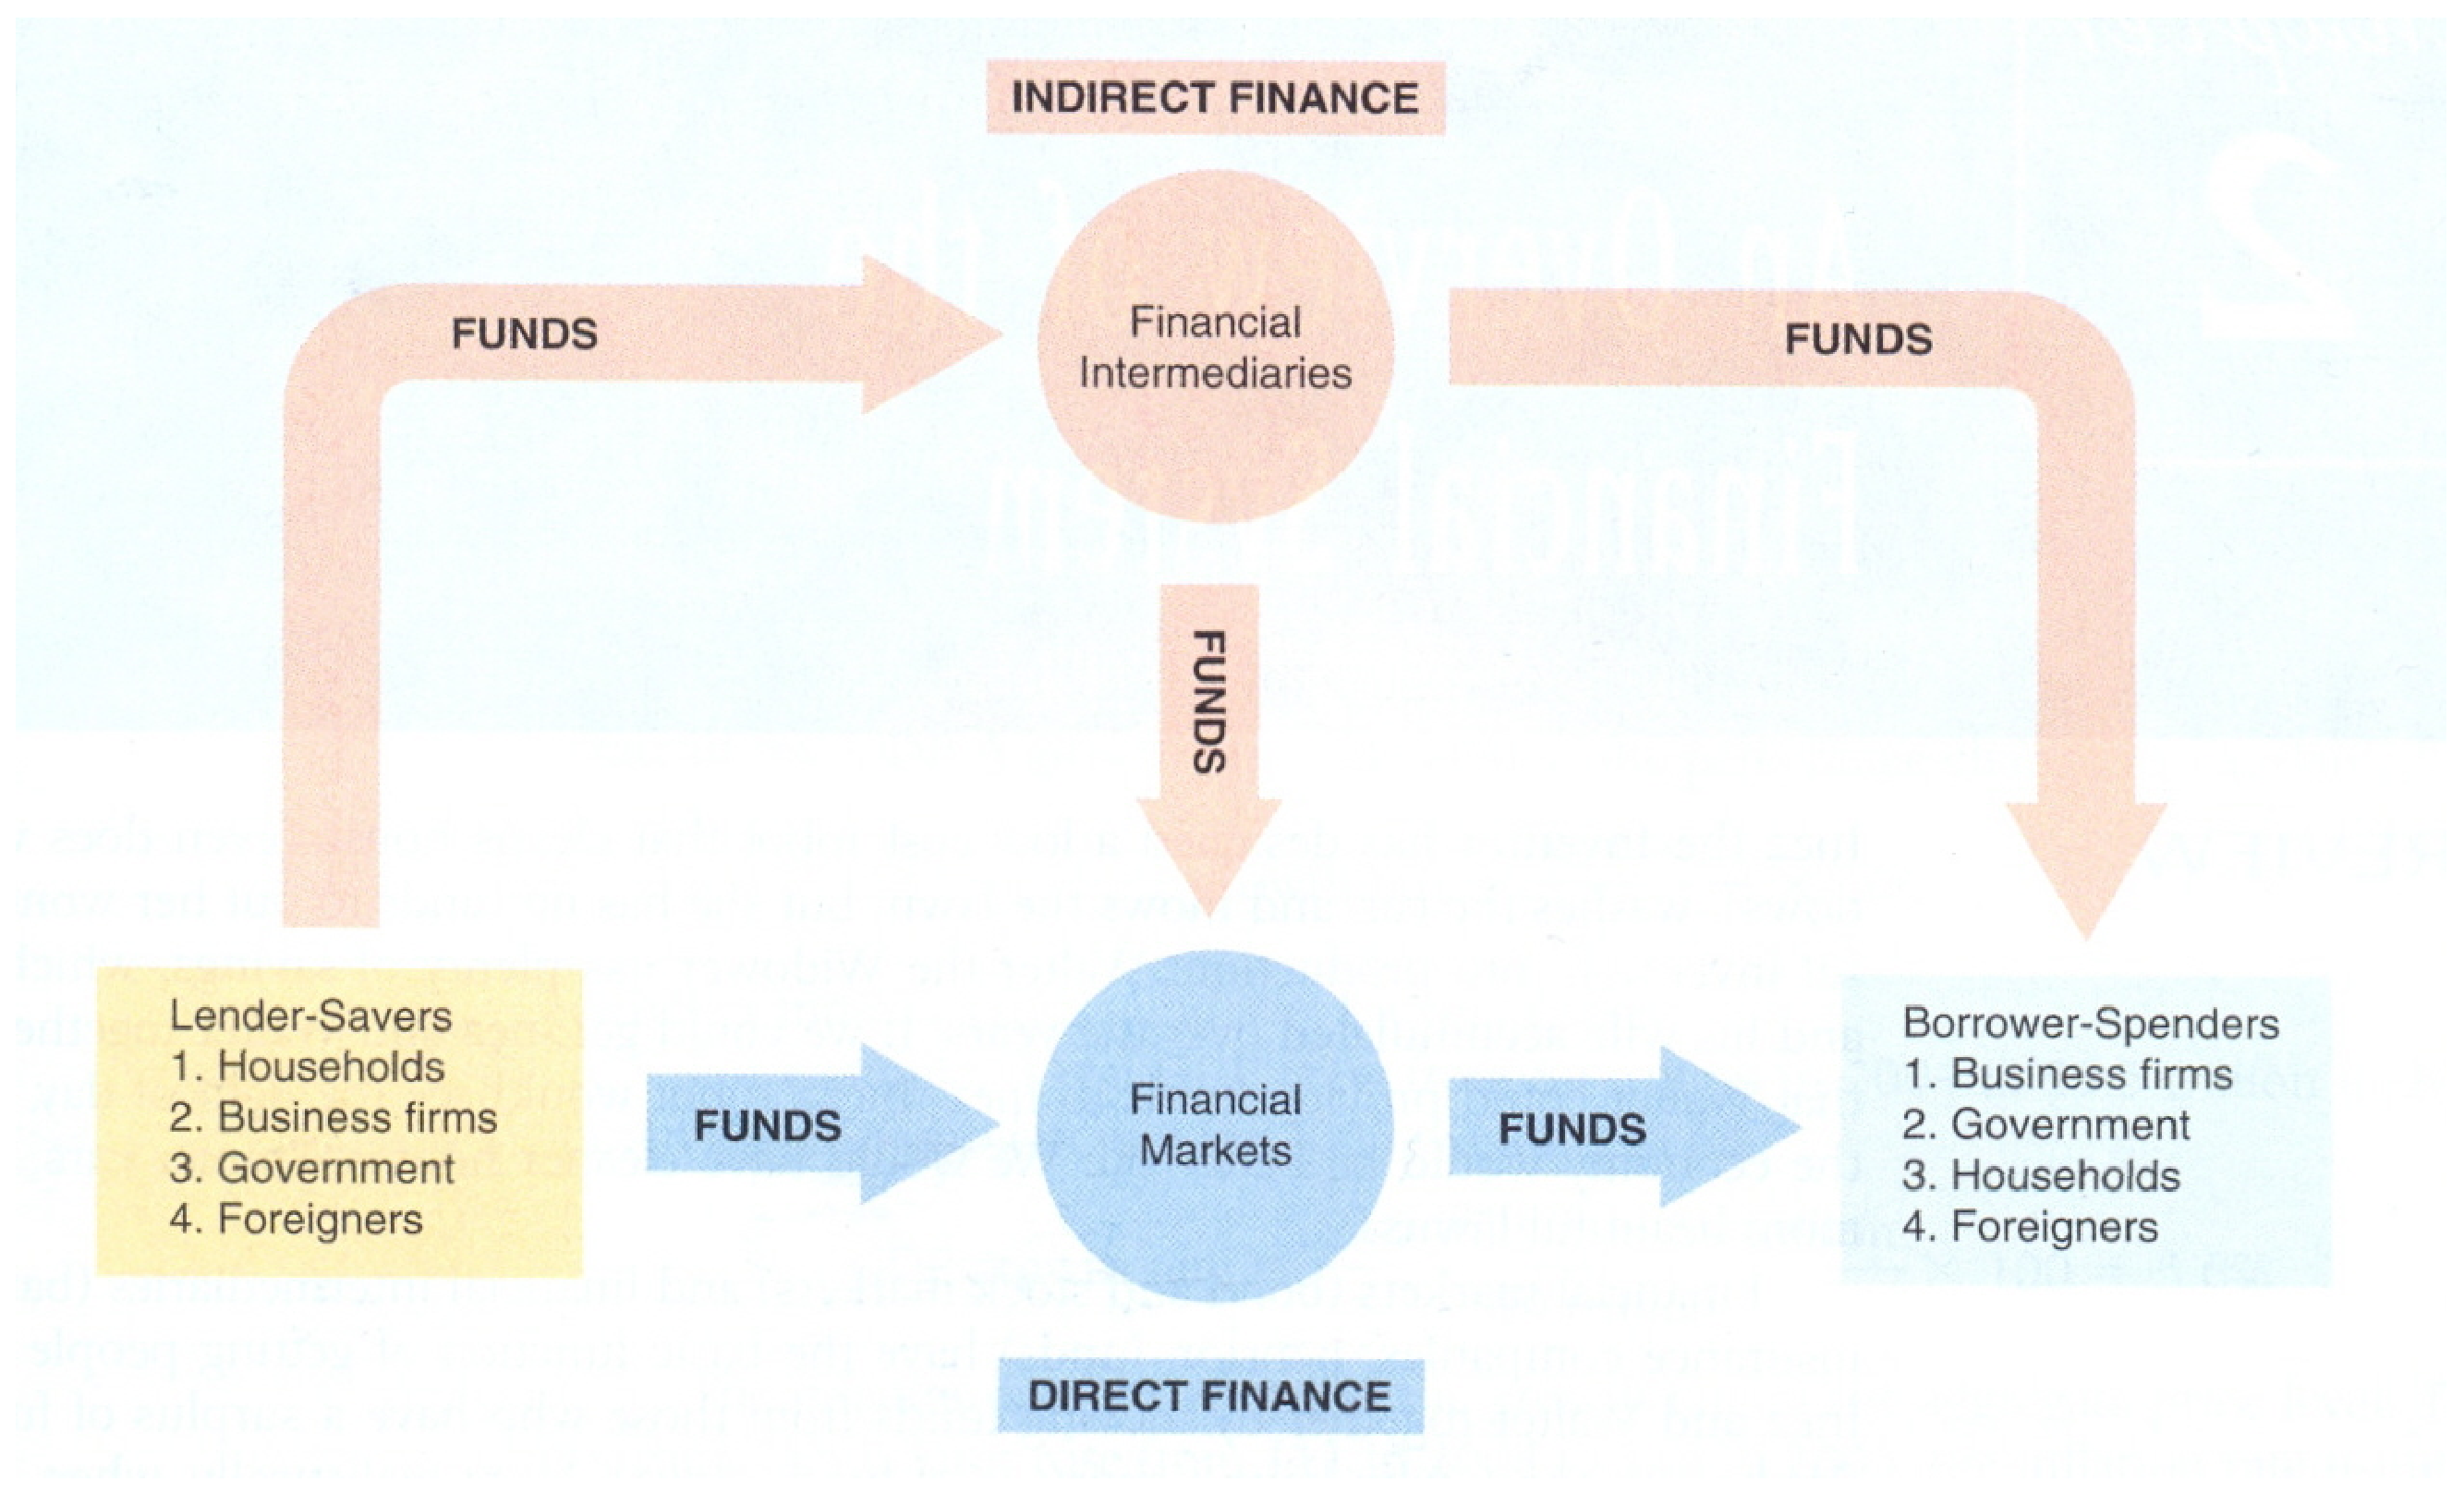
\includegraphics[width=0.8\textwidth]{Figures/intermediates.eps}
\end{figure}
\end{frame}

%==================================================================================
\begin{frame}
\frametitle{Financial intermediaries}
\framebox{Examples}
\hfill \break
\begin{itemize}
\item  Financial advisors
\item  Credit Union
\item Mutual funds/Investment trusts
\item  Insurance Companies
\item Pension funds
\item Commercial banks
\item Investment banks
\end{itemize}

\end{frame}

\begin{frame}
\frametitle{Financial intermediaries}
\begin{itemize}
\item Transform assets
\item Manage risks
\item Process information and monitor borrowers
\item Offer access to a payment system, public good
\end{itemize}


\framebox{Why care?} \hfill \break
\begin{itemize}
\item Facilitate economic growth: mobilising savings so that consumption can be higher in the future as a result of investments made today.
\item Global growth: Sending savings from countries with little room for further investment, to countries with more room than current savings can
satisfy.
\end{itemize}
\end{frame}


\begin{frame}
\frametitle{Why regulate?}

\textit{"We regulate finance over and above the way we regulate
other industries because finance exhibits market failures
that can have devastating consequences"}
\hfill \break
\begin{itemize}
\item financial market malfunction $\rightarrow$ the real economy $\Downarrow$
\item Example: Global financial crisis was triggered by problems in the US subprime mortgage market, but it led to German GDP shrinking by 6 percent in the first quarter of 2009 and the biggest drop in global trade since the 1930s.
\end{itemize}

\end{frame}
%-------------------------------------------------------------
\begin{frame}
\frametitle{Why regulate?}

Two principal drivers of market failures in finance that require
regulation
\textit{....there are others as well}
\hfill \break
\begin{itemize}
\item  Asymmetrical information
\begin{itemize}
\item Consumer protection - balance the interests of unsophisticated consumers of financial products and their sophisticated sellers
\end{itemize}
\item Social externalities
\begin{itemize}
\item  overall consequence of an activity is not captured
by the private interests of those involved in the activity.
\item $\rightarrow$ internalise with social taxes? (Pigouvian reponse)
\item .. costs of financial system failures are $>$ costs to the shareholders of a bank failure. $\Rightarrow$ regulatory
response: provide government insurance for depositors and higher capital requirements than banks would otherwise wish to hold
\end{itemize}
\end{itemize}
\end{frame}



%---------------------------------------------------------------------------
\begin{frame}
\frametitle{Banks are different}
\begin{itemize}
\item Banks accept \textit{deposits}
\item Banks lend to each other
\begin{itemize}
\item Bank A may borrow from Bank B to lend one of its customers a loan to
buy a car from a customer of Bank B.... \\
\framebox{why does this matter?}
\item when one shoe shop fails it might be good for another shoe shop (they do not lend to each other)
\item Failure of one bank $\rightarrow$ undermine other banks
\item Bank runs
\item A single bank failure could lead to a collapse of the financial system
\end{itemize}
\end{itemize}
\end{frame}


%__________________________________________________________________


\begin{frame}
\frametitle{Types of regulatory instruments}
\begin{itemize}
\item ceilings on deposit interest rates
\item restrictions on entry, size, and mergers
\item investment restrictions
\item deposit insurance
\item capital requirements
\item monitoring and bank supervision
\end{itemize}
\end{frame}

%--------------------------------------------------------------------------------


\section{Why Financial Intermediaries Matter}
%
%==================================================================================
%\begin{frame}
%	\begin{center}
%		\centering{\Large The Architecture of Financial Regulation\\ Chapter 1: Regulating Wall Street}
%	\end{center}
%\end{frame}

% --------------------------------------------------------------------------------

\begin{frame}

\frametitle{The Architecture of Financial Regulation}
There are four pillars of financial regulation:
\begin{itemize}\itemsep10pt
\item Encourage innovation and efficiency
\item Provide transparency
\item Ensure safety and soundness
\item Promote competitiveness in global markets
\end{itemize}
		\end{frame}

% --------------------------------------------------------------------------------

\begin{frame}
\frametitle{Limitations of Regulation}
Limitations to regulating the financial system:
\begin{itemize}\itemsep10pt
\item Asymmetric information\\
\quad \quad George Akerlof: Lemon's market
\item Costly state verification\\
\quad \quad Robert Townsend: no disclosure until default, then full disclosure
\item Missing markets\\
\quad \quad Public goods: non-excludable/-diminishable/-rejectable
\end{itemize}
\end{frame}

%-----------------------------------------------------------------
%
% \begin{frame}
% \frametitle{Alternatives to regulation}
% Alternative approaches to financial regulation:
% \begin{itemize}\itemsep10pt
% \item Laissez-faire modification [Preferred by Wall-Street]
% \item Glass-Steagall approach [Preferred by Interventionists]
% \item Carve outs
% \item Limit the size of financial conglomerates
% \end{itemize}
% \end{frame}

% ------------------------------------------------------------------

\begin{frame}
\begin{enumerate}
\item Modification of laissez-faire approach:
\begin{itemize}
\item Create appropriate tools for systemic risk regulation
\item Price implicit public subsidies
\item Create bankruptcy tools
\end{itemize}
\vspace{3mm}
\item Glass-Steagall approach:
\begin{itemize}
\item Legacy investment banks are converted into bank holding companies
\item Reverts them into broker-dealer status
\end{itemize}
\vspace{3mm}
\item Carve outs:
\begin{itemize}
\item Management of in-house hedge funds
\item Creation of off-balance-sheet affiliates
\item Large propriety trading positions in cash securities and derivatives
\item Principal investors in non-financial activities
\end{itemize}
\vspace{3mm}

\item Limit the size of financial conglomerates that incorporate commercial banking units
\end{enumerate}
\end{frame}

% --------------------------------------------------------------------------------

\begin{frame}
\frametitle{\insertsection}
\textbf{a) Reducing Transaction Costs}
\begin{itemize}
\item FI have \textit{economies of scale}:
\par\smallskip
getting information about demanded and provided funds, assessing risks, bargaining, designing and enforcing contracts, buying/selling stock shares -- these tasks can be accomplished by FI with much lower transaction costs by specialized information processing abilities, large transaction volumes, specific human capital (expertise)
\item FI have \textit{economies of scope}:
\par\smallskip
FI provide additional services like risk diversification, optimizing portfolios, and consulting. Sometimes these services need the same infrastructure and the same human capital. Hence it \textit{may} reduce cost when one FI provides these services.
\end{itemize}
\end{frame}

% --------------------------------------------------------------------------------

\begin{frame}
\frametitle{\insertsection}
\textbf{b) Dealing with Risk:}
\begin{itemize}
\item Risks: Investment projects may fail, borrowers may become insolvent.
\item Reducing the risk by pooling them, reducing the risks arising from asymmetric information problems (see below).
\item Reducing the risk by selling assets with differert risk/return structures which are prefered by the
lender/saver (asset transformation, e.g. time deposit, fund shares).
\item Trading risky assets means that also risks are traded, all prices contain a ``risk premium''.
\end{itemize}
\end{frame}

% --------------------------------------------------------------------------------


\begin{frame}
\frametitle{\insertsection}
\textbf{c) Dealing with asymmetric information}
\begin{itemize}
\item \textbf{Adverse Selection:}
\begin{itemize}
\item Hidden characteristics of a potential borrower (e.g.) before a contracting.
\item Borrower knows his risk better than the lender.
\item If lender offers a contract which is optimal for a borrower with average risks, this may be unattractive for those with good risks. This may result in a market failure.
\end{itemize}

\item \textbf{Moral Hazard:}
\begin{itemize}
\item Hidden action of a borrower (e.g.) after contracting.
\item Borrower tales the money to engage in a prject that is undesireable for the lender. This reduces the probability for a successfully returned credit.
\end{itemize}

\item FI may alleviate this problem e.g. by screening, collaterals, optimal design of contracts. Again, they have the resources to do that with low transaction costs.
\end{itemize}
\end{frame}

% --------------------------------------------------------------------------------

\begin{frame}
\frametitle{\insertsection}

\textbf{Depository institutions (banks):}
\begin{itemize}
\item Accept deposits from individuals and institutions as liabilities, providing loans and mortgages as assets.
\item Example: Commercial banks, thrifts (saving and loans associations, mutual saving banks, credit unions).
\end{itemize}
% Deutsche Bank, Commerzbank, LBS

\textbf{Contractual savings institutions:}
\begin{itemize}
\item Accept premiums and contributions from government, firms and individuals as liabilities, investment in bonds, stocks and government securities.
\item Example: life insurance, pension funds, retirement funds
\end{itemize}
% Allianz, Debeka

\textbf{Investment intermediates:}
\begin{itemize}
\item Selling commerical stocks, bonds or shares as liabilities, providing business loans and investment in stocks and bonds as assets.
\item Example: Finance companies, mutual funds, private equity funds
\end{itemize}
% Morgan Stanley, Blackstone (in Germany it is part of investment banking)

\end{frame}

\section{Banks as Financial Intermediaries}
%

% ------------------------------------------------------------------
\begin{frame}
\frametitle{What is a balance sheet}
\begin{itemize}
\item A summary of the assets and liabilities of a business (bank)
\item A snapshot of assets and liabilities at a particular point in time
\item A balance sheet always balances - double entry bookkeeping
\begin{itemize}
\item Assets are \textit{owned} by the bank
\item Liabilities are \textit{owed} by the bank
\end{itemize}
\end{itemize}

\end{frame}

% ==================================================================
\begin{frame}
\frametitle{\insertsection}

\begin{center}
\textit{The Bank's Balance Sheet}
\end{center}
\par\medskip

\begin{tabular}{l|l}
\hline
Assets & Liabilities\\
\hline
\begin{minipage}{5cm}
\begin{itemize}
\item Reserves {\small (required, excess)}
\item Cash
\item Securities/Bonds
\begin{itemize}
\item firm bonds
\item governmental bonds
\end{itemize}
\item Loans
\begin{itemize}
\item industrial
\item consumer
\item real estate
\item inter-bank
\item other
\end{itemize}
\item Other assets\\
{\small (e.g. physical assets)}
\end{itemize}
\end{minipage}
&
\begin{minipage}{5cm}
\begin{itemize}
\item (Checkable) Overnight deposits
\item Nontransaction desposits
\begin{itemize}
\item Time deposits
\item Redeemable deposits\\(saving accounts)
\end{itemize}
\item Borrowings
\begin{itemize}
\item Inter-bank loans
\item Central bank loans
\item Other
\end{itemize}
\item Bank Capital
\end{itemize}
\end{minipage}\\
\hline
\end{tabular}
\end{frame}

% =================================================================
%
\section{Banks as financial intermediaries}
%
% =================================================================


%-----------------------------------------------------------------
\begin{frame}
  \begin{center}
    {\Large \textbf{Frictions in Financial Markets}}
  \end{center}
\end{frame}
%-----------------------------------------------------------------

\begin{frame}
\frametitle{\insertsection}

\textbf{a) Liquidity Management}

\begin{itemize}
\item For deposit outflows the bank needs liquid assets like cash or reserves.

\item If there are not enough liquid positions on the asset side the bank needs expensive overnight loans or has to sell other assets, or it becomes illiquid. These are costs of deposit outflows.

\item Problem: If customers receive a signal of liquidity problems they also wish to draw their deposits. This enforces the liquidity problem and may lead to bankruptcy.

\item Liquidity management has to balance the liquidity of assets with the deposit position on the liability side. More generally: Given a probability distribution of inflows and outflows on the liability side, the asset side should be structured to meet the obligations to the depositors.
\end{itemize}
\end{frame}

% ------------------------------------------------------------------

\begin{frame}
\frametitle{\insertsection}

\begin{itemize}
\item The higher the expected deposit outflows  and/or the higher the cost of deposit outflows are the more excess reserves are required.
\end{itemize}
\par\medskip

\textbf{b) Asset Management }

\begin{itemize}
\item Management of risk and return of the assets (portfolio approach). Finding the mix of risky and riskless assets with the highest expected utility (assumption: risk aversion).

\item The liquidity considerations (see a)) can be seen as an additional restriction to portfolio management.

\item Portfolio theory is a core concept in (financial) economics. Details are given in the next subsection.
\end{itemize}
\end{frame}

% ------------------------------------------------------------------

\begin{frame}
\frametitle{\insertsection}

\textbf{c) Liability management}

\begin{itemize}
\item Deposits are not ``given'' and not the only source of funds. Decision how to acquire which types of liabilities.

\item Differences of liabilities:
\begin{itemize}
\item Hows fast could an additional liability be acquired?
\item Probability of outflows
\item Costs = interest rates (e.g. for time deposits, for inter-bank or central bank loans)
\end{itemize}

\item Development of new financial instruments (e.g. certificates of deposits (CD) which are similar to bonds)
\end{itemize}

\end{frame}

% ------------------------------------------------------------------

\begin{frame}
\frametitle{\insertsection}

\textbf{d) Bank Capital Management}

\begin{itemize}
\item Most assets have risks: Credits may fail, bonds prices may fall. Hence, the value of the asset side is volatile.

\item With a certain probability the losses of the asset side may exceed the bank capital: the bank becomes insolvent.

\item Actual development: Large bank crisis in the USA in 2008. About 500 Billion Dollar asset values (especially housing loans and mortgages) had to be written off.

\item The higher the bank capital (in percent of the liability side), the lower is the risk of insolvency.

\item But: The return on equity (RoE) of the bank owners (return on assets / bank capital) is c.p. lower when the bank capital has a higher share of the liability side $\rightarrow$ trade-off!
\end{itemize}

\end{frame}


% =================================================================
%
\section{Adverse Selection Problems}
%
% =================================================================
\begin{frame}
\frametitle{\insertsection}

\textbf{Information Asymmetries:}
\small
\begin{itemize}
\item before contracting: hidden characteristics $\rightarrow$ adverse selection
\par\medskip
\begin{itemize}
\item buying shares or bonds of a firm $\Rightarrow$ characteristics are not known to the buyer
\item providing a loan to a borrower with unknown ability to pay back the loan (credit risk)
\par\medskip

\item [$\Rightarrow$] decision is based on expectations about the characteristics
\item [$\Rightarrow$] expectations are built on prior and posterior information
\item [$\Rightarrow$] limited possibilities to reveal the unknown characteristics
\item [$\Rightarrow$] Pooling vs. Separating equilibria
\end{itemize}

\item after contracting: hidden action $\rightarrow$ moral hazard
\par\medskip

Firm uses the funds for financing projects which are more risky than indicated in the negotiation with the  lender or buyer of a share. The latter can not observe this, but they can expect that there is an incentive for moral hazrd.
\end{itemize}
\end{frame}

% ------------------------------------------------------------------

\begin{frame}
\frametitle{\insertsection}

The original version: Market for used cars
\begin{figure}
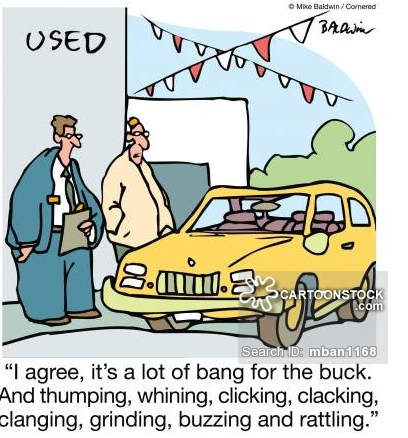
\includegraphics[width=0.6 \textwidth]{Figures/Cars.png}
\end{figure}
\end{frame}


\begin{frame}
\frametitle{Market for used cars}
\begin{itemize}
\item Cars have a different quality $q$ (from ``very good'' $q=b$ to ``bad'' $q=0$, bad cars = ``lemons'')
\item The seller is privately informed about the quality $q\in[0,b]$.
\item The seller will accept any price $p\geq q$.
\item The buyer is willing to pay any price $p\leq \alpha\cdot q$ with $\alpha>1$.
\item For any given $q$ there exists a price $\in[q,\alpha q]$ where buyer and seller mutually benefit from the deal.
\par\medskip

\item \textbf{But:} The buyer is not able to observe $q$\\ $\Rightarrow$ building expectations $E[q]$.
\end{itemize}

\end{frame}

% ------------------------------------------------------------------

\begin{frame}
\frametitle{\insertsection}

Assume that the quality $q$ is \textit{uniformly distributed} on $[0,b]$. This is known by the buyer.
For any used car the expected quality is hence $E[q]=b/2$. Therefore
$$
p(E[q])\leq \alpha\cdot\frac{b}{2}
$$

Two cases:
\begin{itemize}
\item \textit{Case 1:} $\alpha \geq 2$. Then the buyer is willing to pay $p\geq b$ and all cars will be sold.
\item \textit{Case 2:} $1<\alpha<2$. Then the market breaks down!
\end{itemize}

\end{frame}

% ------------------------------------------------------------------

\begin{frame}
\frametitle{\insertsection}

Market breakdown:
{\small
\begin{itemize}
\item For $\alpha<2$ the buyer will never pay $p=b$.
\item No high quality cars ($q=b$) will be sold. They can be removed from the interval (e.g. $q\in[0,b-\epsilon]$).
\item This can be anticipated by the buyer. The expected average quality decreases (e.g. $E[q]=(b-\epsilon)/2$).
\item The willingness to pay also decreases.
\item The remaining best quality cars leave the market.
\item and so forth... (``race to the bottom'')
\end{itemize} }
\end{frame}

% ------------------------------------------------------------------

\begin{frame}
\frametitle{\insertsection}

\textbf{Financial Markets:}

\begin{itemize}
\item Firm needs funds to finance a risky project. The funds can be obtained by debt or equity. Assume that the firm demands for a loan $L$.

\item The (risk neutral) firm is willing to pay an interest rate $i_L$ which does not exceed the expected return of the project $r$.

\item The bank will provide the loan $L$ when the interest rate covers at least the interest rate for a secure asset $i_S$ plus the risk premium $RP$.

\item Assume that the loan is either returned successfully with probability $1-p$ or it fails completely with probability $p$. The minimum risk premium is therefore:
\begin{align}
L(1+i_S) &= L(1+i_L)(1-p)+0\cdot p\\
\Rightarrow\quad
RP=i_L-i_S &= \frac{p}{1-p}(1+i_S)
\end{align}

\end{itemize}

\end{frame}

% ------------------------------------------------------------------

\begin{frame}
\frametitle{\insertsection}

\begin{itemize}
\item Problem: $p$ is \textit{private information} of the firm = not known by the bank!

\item Offering a loan contract with an interest rate $i_L$ (and risk premium) based on the \textit{expected} probability $E[p]$ taken from a prior distribution of risks.

\item Typically the expected return and the risk of investment projects are positively correlated.
Firms with \textit{profitable low risk projects} with
$$
r<i_S+\frac{E[p]}{(1-E[p])}(1+i_S)
$$
will not get a loan contract!

\item The remaining projects are hence more risky which leads to an increase of $E[p]$ $\Rightarrow$ a similar mechanism as in the ``market for lemons'' example applies.
\end{itemize}

\end{frame}

% ------------------------------------------------------------------

\begin{frame}
\frametitle{\insertsection}

\textbf{Credit Rationing:}
\par\medskip

Adverse Selection Effect: With an increasing interest rate more and more good (= low risk) projects leave the market and the expected risk increases:
$$
E[p]=E[p(i_L)],\qquad \frac{dE[p(i_L)]}{di_L}>0
$$
Profit maximizing bank:
\begin{align}
\max_{i_L} \pi &= (1-E[p(i_L)])(1+i_L)L\\
\Rightarrow\quad
\frac{d\pi}{di_L} &= -\frac{dE[p(i_L)]}{di_L}(1+i_L)L+(1-E[p(i_L)])L=0\\
\Rightarrow\quad
i_L^* &= \frac{(1-E[p(i_L)])-\frac{dE[p(i_L)]}{di_L}}{\frac{dE[p(i_L)]}{di_L}}
\end{align}
\end{frame}

% ------------------------------------------------------------------

\begin{frame}
\frametitle{\insertsection}

What are the consequences?

\begin{itemize}
\item The profits do not monotonously increase with market interest rate $i_L$.

\item If loans demand increases \textit{there is not neccessarily a Walrasian adjustment of the equilibrium interest rate! }

\item The demand side of the loans market will be rationed.

\item Existence of \textit{rationing equilibria}.

\item The notional plans of the firms cannot be fulfilled \\
$\Rightarrow$ spillover to other markets
\begin{itemize}
\item  e.g. markets for bonds or equities to finance the project
\item  e.g. markets for investment goods
\end{itemize}

\end{itemize}

\end{frame}

% ------------------------------------------------------------------

\begin{frame}
\frametitle{\insertsection}

There are different ways how to solve or to alleviate the problem:

\begin{itemize}
\item Providing  better information = decreasing information asymmetry
\begin{itemize}
\item \textit{Screening:} The less informed agent has an incentive
\begin{itemize}
\item     to collect information by himself
\item     to buy additional information supplied by other agents
\item     to provide different contracts with self-selection effects
\end{itemize}
\item \textit{Signalling:} The privately informed agent has an incentive to provide a trustworthy (costly) signal about his characteristics.
\item \textit{Governmental Regulation}
\end{itemize}

\item Collateral and Net Worth
\par\smallskip
  The information asymmetry is not resolved but has minor consequences since in case of a failed project the return of the loan do not fail.
\end{itemize}

\end{frame}

% ------------------------------------------------------------------

\begin{frame}
\frametitle{\insertsection}

\textbf{Screening by collecting information}

\begin{itemize}
\item High information costs, especially for lenders with low expertise.

\item Bank as a financial intermediate with expertise and specialized human capital reduces such information costs:
\begin{itemize}
\item Multiple lender of funds $\Rightarrow$ bank deposits
\item Bank is pooling the risks and guarantees the depositor an interest rate
\item Screening costs of multiple non-specialized lenders are reduced and transferred to the bank
\item The bank as the intermediate lender faces a lower information asymmetry
\end{itemize}

\item The existence of a professional banking system is a prerequisite for a working credit market (crucial for developing countries).
\end{itemize}
\end{frame}

% ------------------------------------------------------------------

\begin{frame}
\frametitle{\insertsection}

\textbf{Screening by buying information provided by others}

\begin{itemize}
\item Rating agencies (e.g. Standard \& Poors, Moody): (Large) Borrowers are rated according to a standardized scale (see Mishkin (2006), chapter 6, p.123)

% \item In Germany: SCHUFA (Schutzgemeinschaft für allgemeine Kreditsicherung)
\end{itemize}

\textbf{Problems:}

\begin{itemize}
\item \textit{Free-rider problem} since information is a non-rival good. Once, when information is made public, there is no incentive anymore to pay for it.

\item How \textit{trustworthy} is that information?  Moral Hazard problem of information providing institutions since the customer (e.g. bank) is not able to asses the reliability of the information.
\end{itemize}
\end{frame}

% ------------------------------------------------------------------

\begin{frame}
\frametitle{\insertsection}

\textbf{Governmental Regulation:}
\par\medskip

If investors need financial funds, e.g. by demanding credits or selling bonds or stocks, they can be forced by law to provide some information to reduce the information asymmetry. E.g.
\begin{itemize}
\item adhere standard accounting principles
\item providing information about the balance sheet and other (financial) indicators like sales, earnings, assets
\item in case of stock markets: publish relevant informations regularly, annual meeting of shareholders etc.
\end{itemize}
\label{govreg}
\end{frame}

% ------------------------------------------------------------------

\begin{frame}
\frametitle{\insertsection}

\textbf{Signalling:}

\begin{itemize}
\item A firm with a low risk project has an incentive to provide a signal so that the lender is informed about the low risk (and charging a low risk premium).

\item If signalling should make sense...
\begin{itemize}
\item[(a)] the signal must  be costly
\item[(b)] there must exist signals that are too expensive for a high risk firm but not too expensive for low risk firms $\Rightarrow$ discrimination is possible.
\end{itemize}

\item Otherwise high risk firms have an incentive to \textit{imitate} the signal so that signalling provides no information (pooling equilibrium).
\end{itemize}
\end{frame}

% ------------------------------------------------------------------

\begin{frame}
\frametitle{\insertsection}

Signalling means ``building reputation''. Reputation signals (e.g.):

\begin{itemize}
\item Loans have been successfully returned in the past.
\item Projects are financed also with equity capital.
\item Firm provides voluntarily more sensitive information than required by law.
\item Firm has valuable assets ($\rightarrow$ similar to collaterals).
\end{itemize}
\par\bigskip

This may be a problem for new and small firms.
\end{frame}

% ------------------------------------------------------------------

\begin{frame}
\frametitle{\insertsection}

\textbf{Collaterals:}

\begin{itemize}
\item In case of failure of the investment project the investor has other assets which can be sold to meet the debt obligations.

\item The borrower must prove that he has such collaterals before signing the credit contract.

\item The credit contract may include the obligation that a certain asset must not sold before the credit is returned successfully.

\item The credit contract includes that lender automatically becomes the owner of an asset in case of a credit failure.

\item The credit contract includes that the lender has property rights on the asset which are returned to the borrower in case of a successfully returned credit $\Rightarrow$ mortgages (e.g. in case of housing, real estate)
\end{itemize}
\end{frame}

% ------------------------------------------------------------------

\begin{frame}
\frametitle{\insertsection}

Collaterals $C$ lower the risk premium:
\begin{align}
L(1+i_S) &=L(1+i_L)(1-p)+pC\\
\Rightarrow\quad
RP=i_L-i_S &=\frac{p}{1-p}(1+i_S)-\frac{p}{1-p}\frac{C}{L}
\end{align}
with $C=\arg\max\{0,(1+i_S)L\}$. In case of $C=L(1+i_S)$ there is no credit risk for the lender anymore.
\par\medskip

\textbf{Problems:}
\begin{itemize}
\item Providing collaterals is costly (e.g. opportunity costs).
\item The access to collaterals is limited (e.g. start-up companies).
\item The value of collaterals may be uncertain (see the recent housing crisis in the U.S. -- dramatic decrease of house prices = decrease of the value of collaterals)
\end{itemize}
\end{frame}

\begin{frame}
  \frametitle{Coordination issues in Banking}
  \begin{center}
    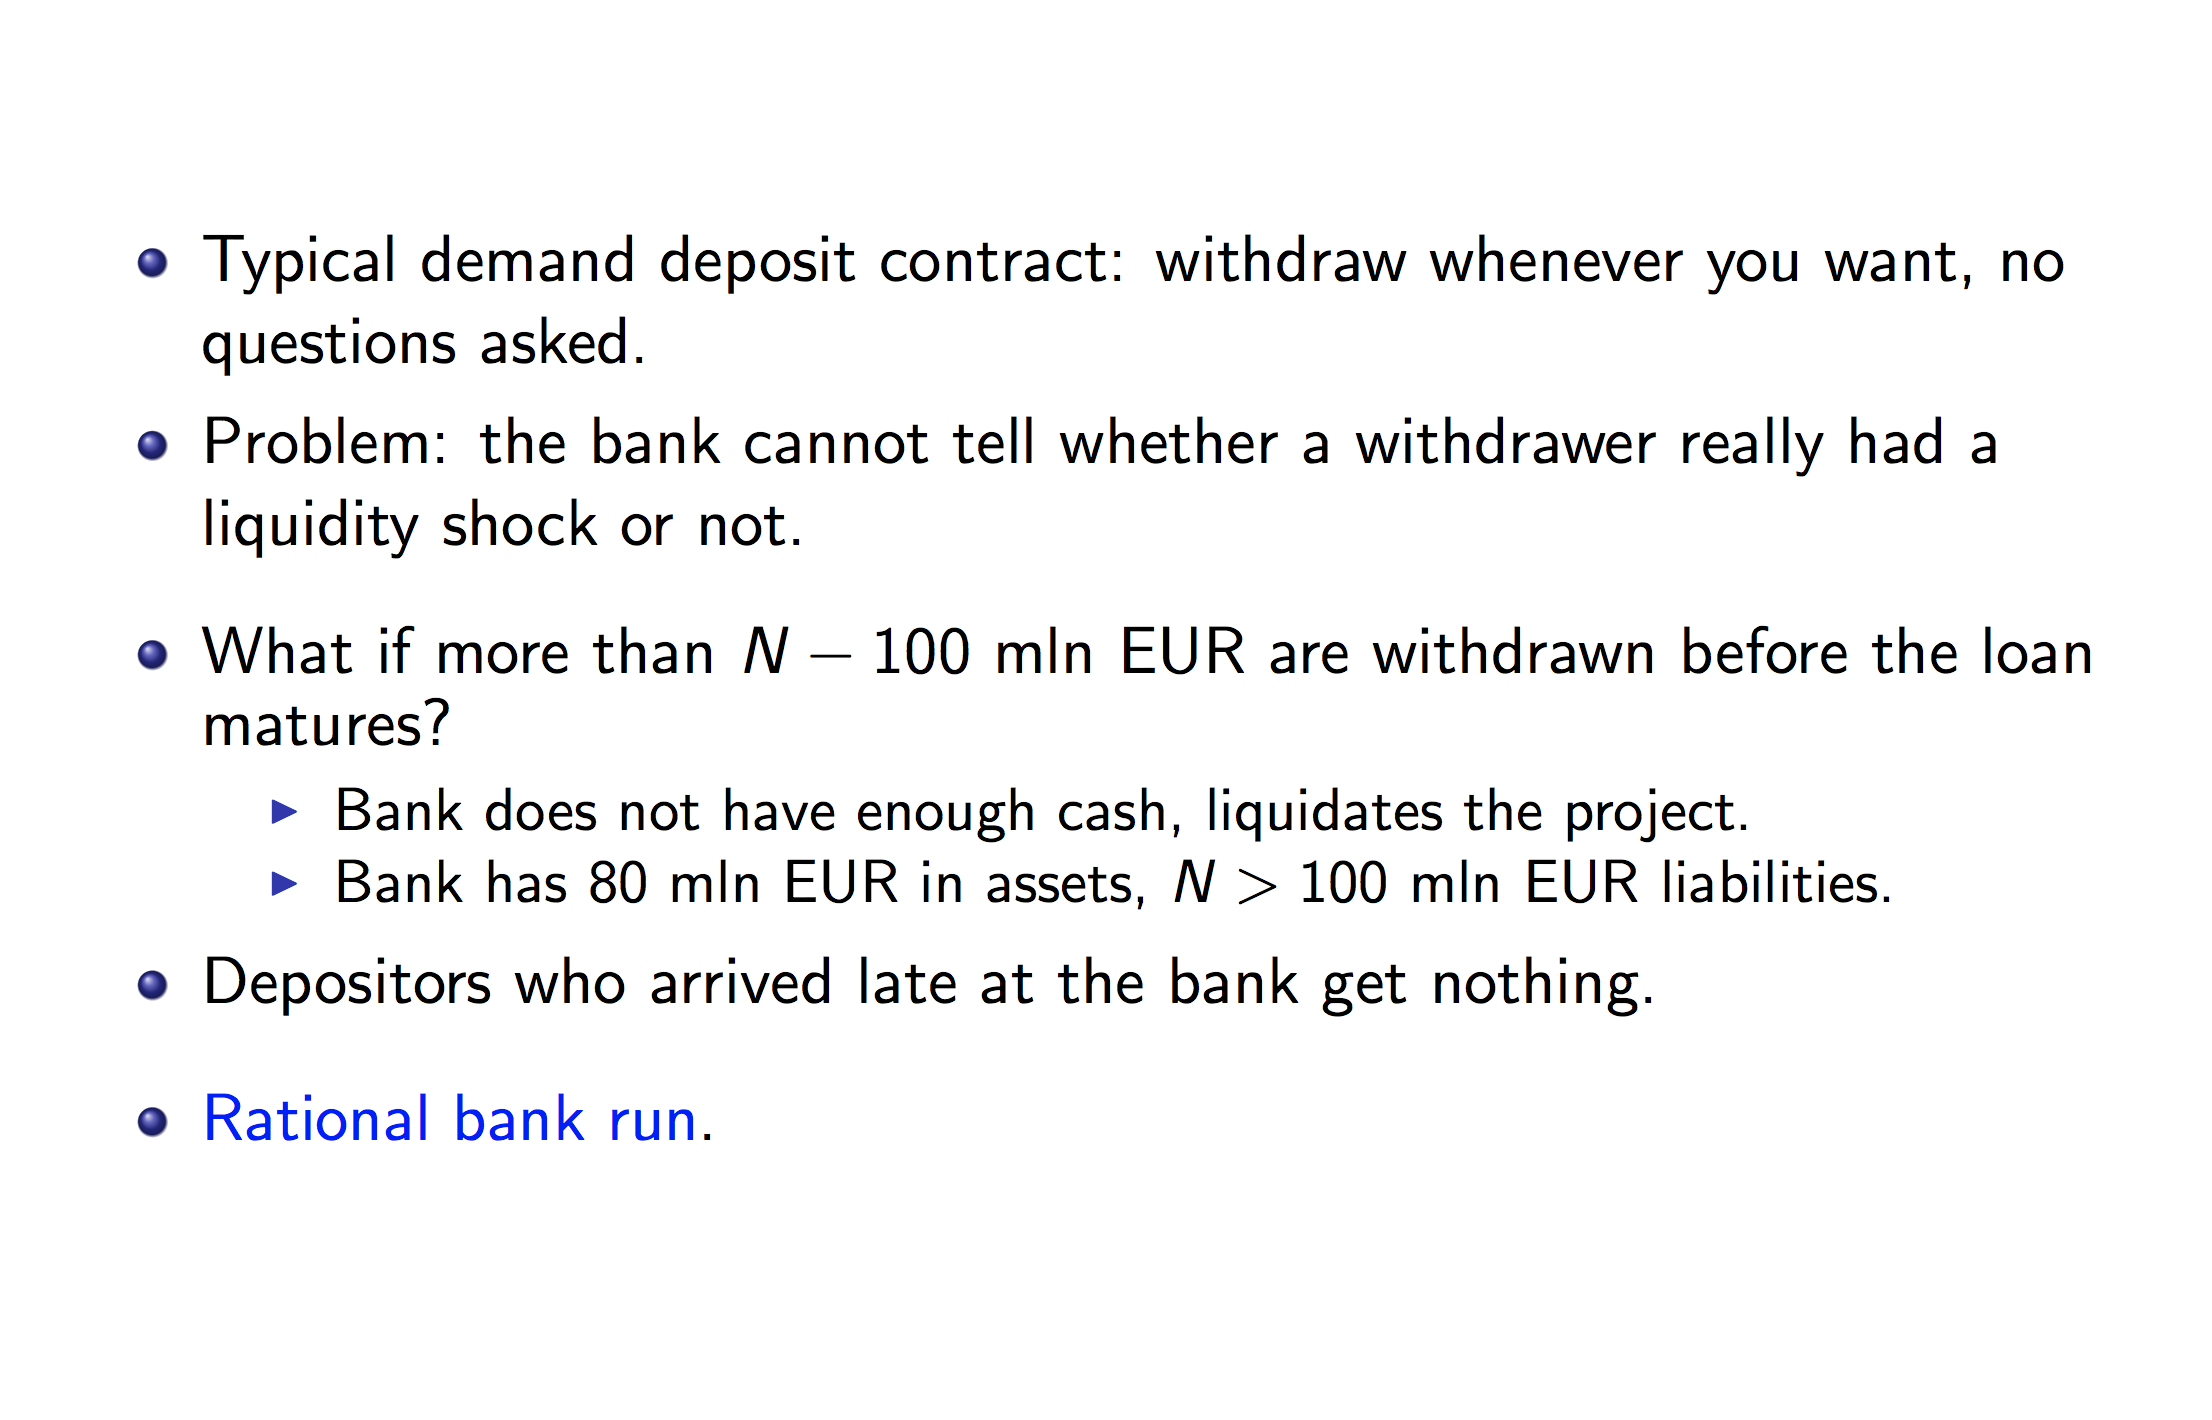
\includegraphics[width=\textwidth]{Figures/bank_runs1.png}
  \end{center}
\end{frame}
\begin{frame}
  \frametitle{Coordination issues in Banking}
  \begin{center}
    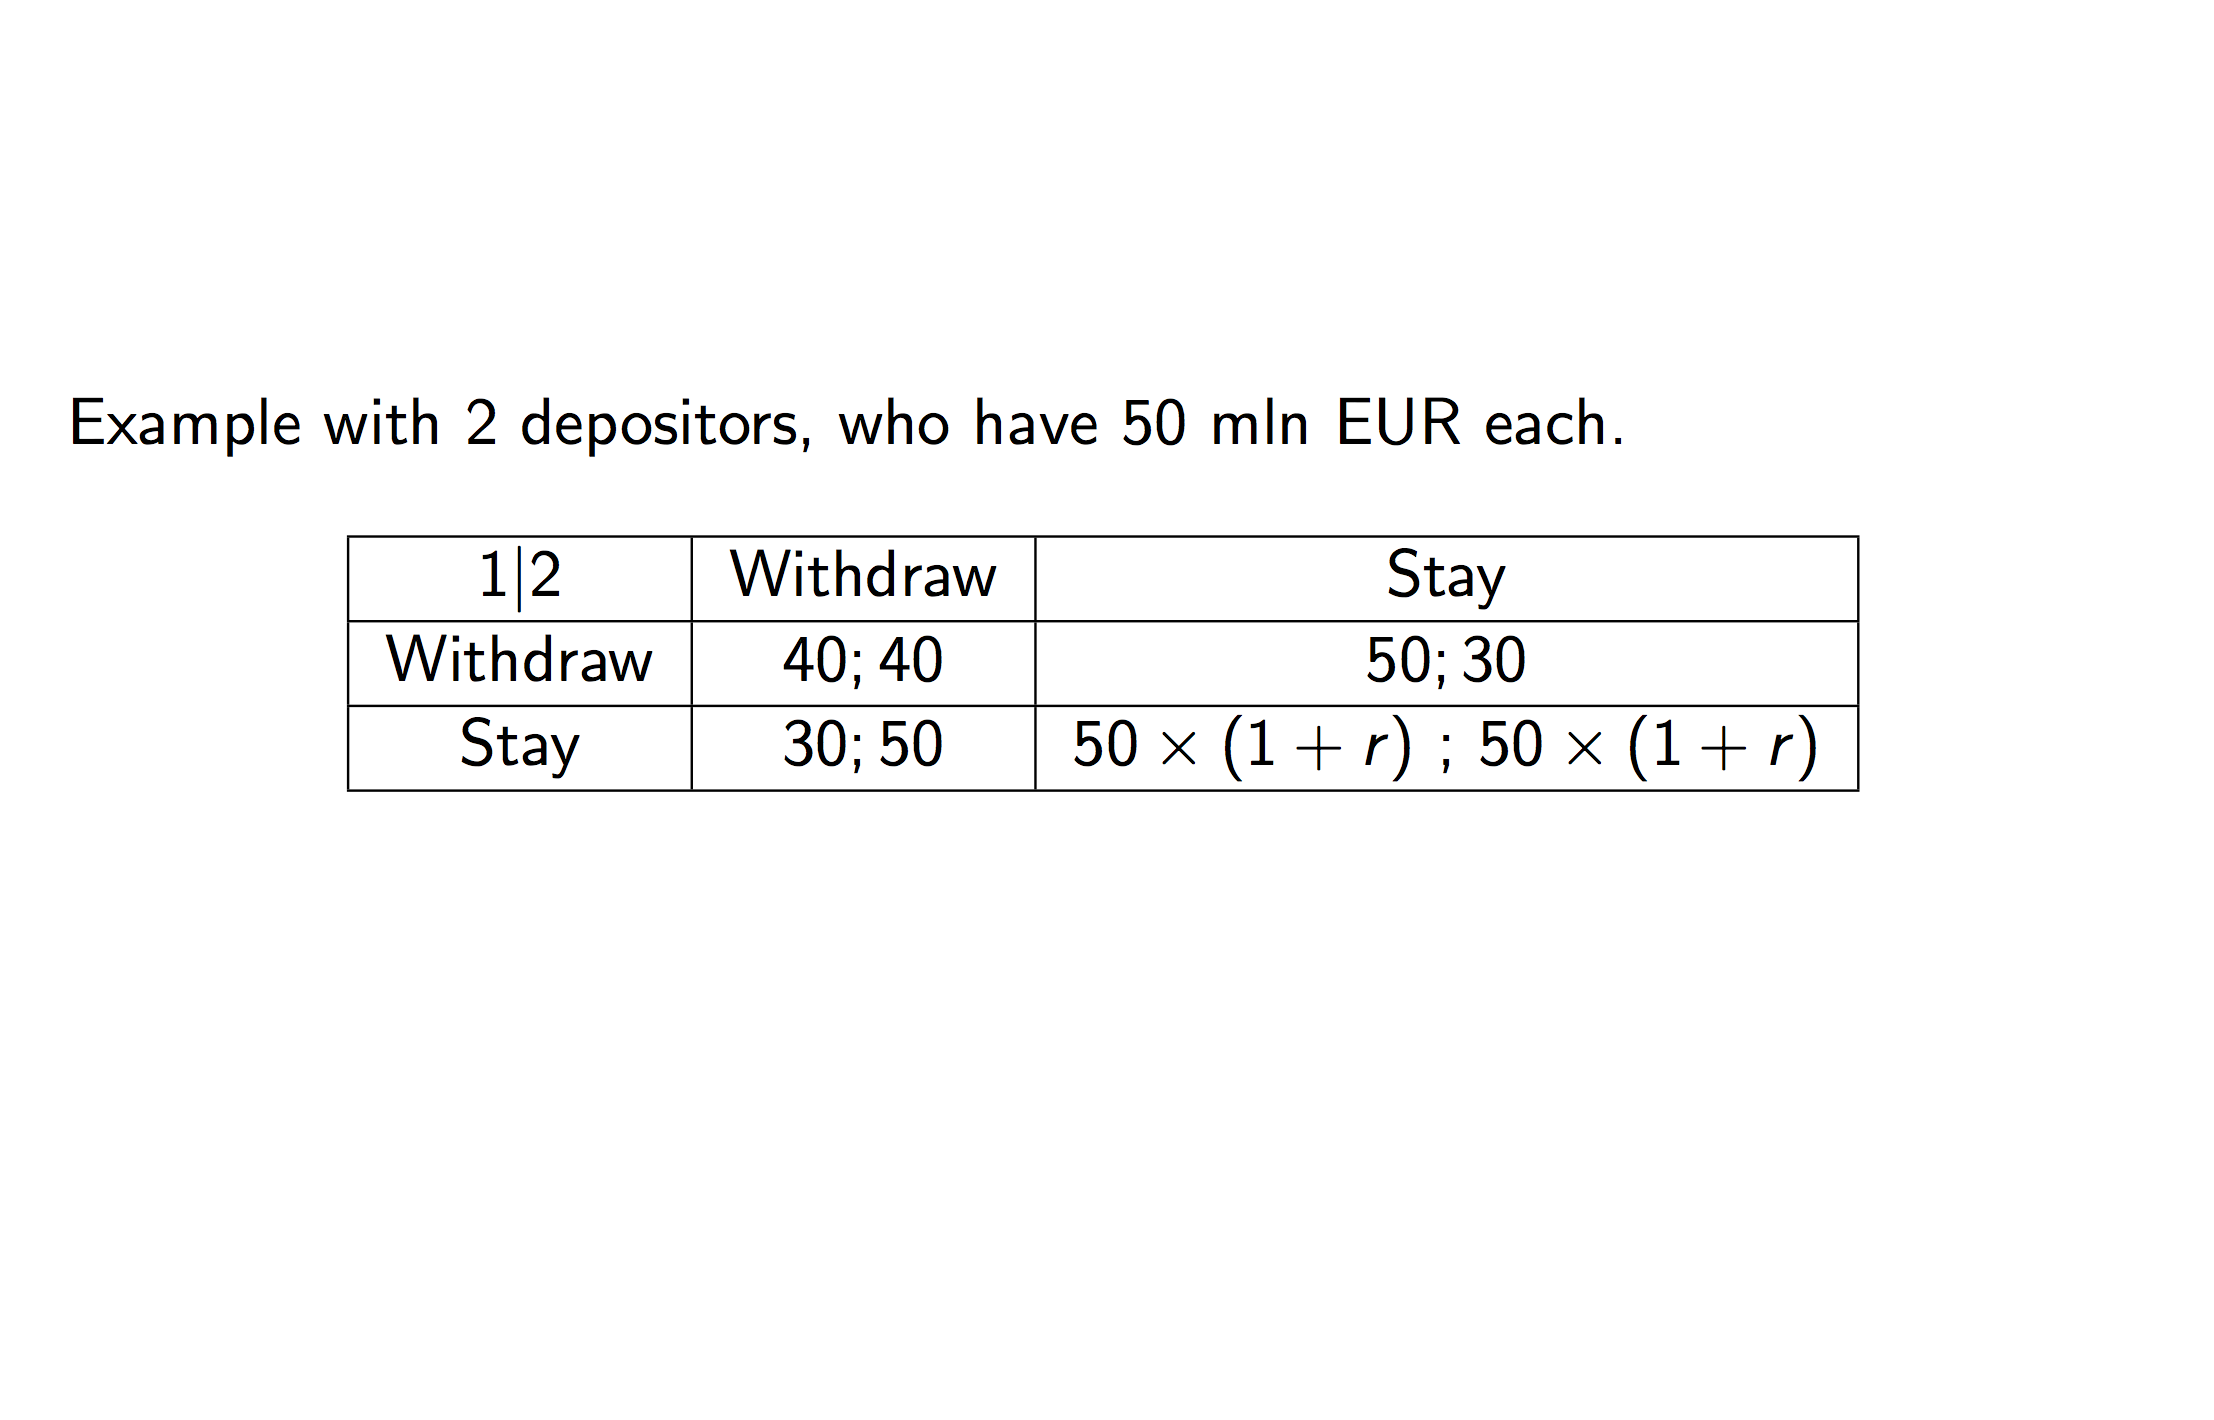
\includegraphics[width=\textwidth]{Figures/bank_runs2.png}
  \end{center}
\end{frame}
\begin{frame}
  \frametitle{Coordination issues in Banking}
  \begin{center}
    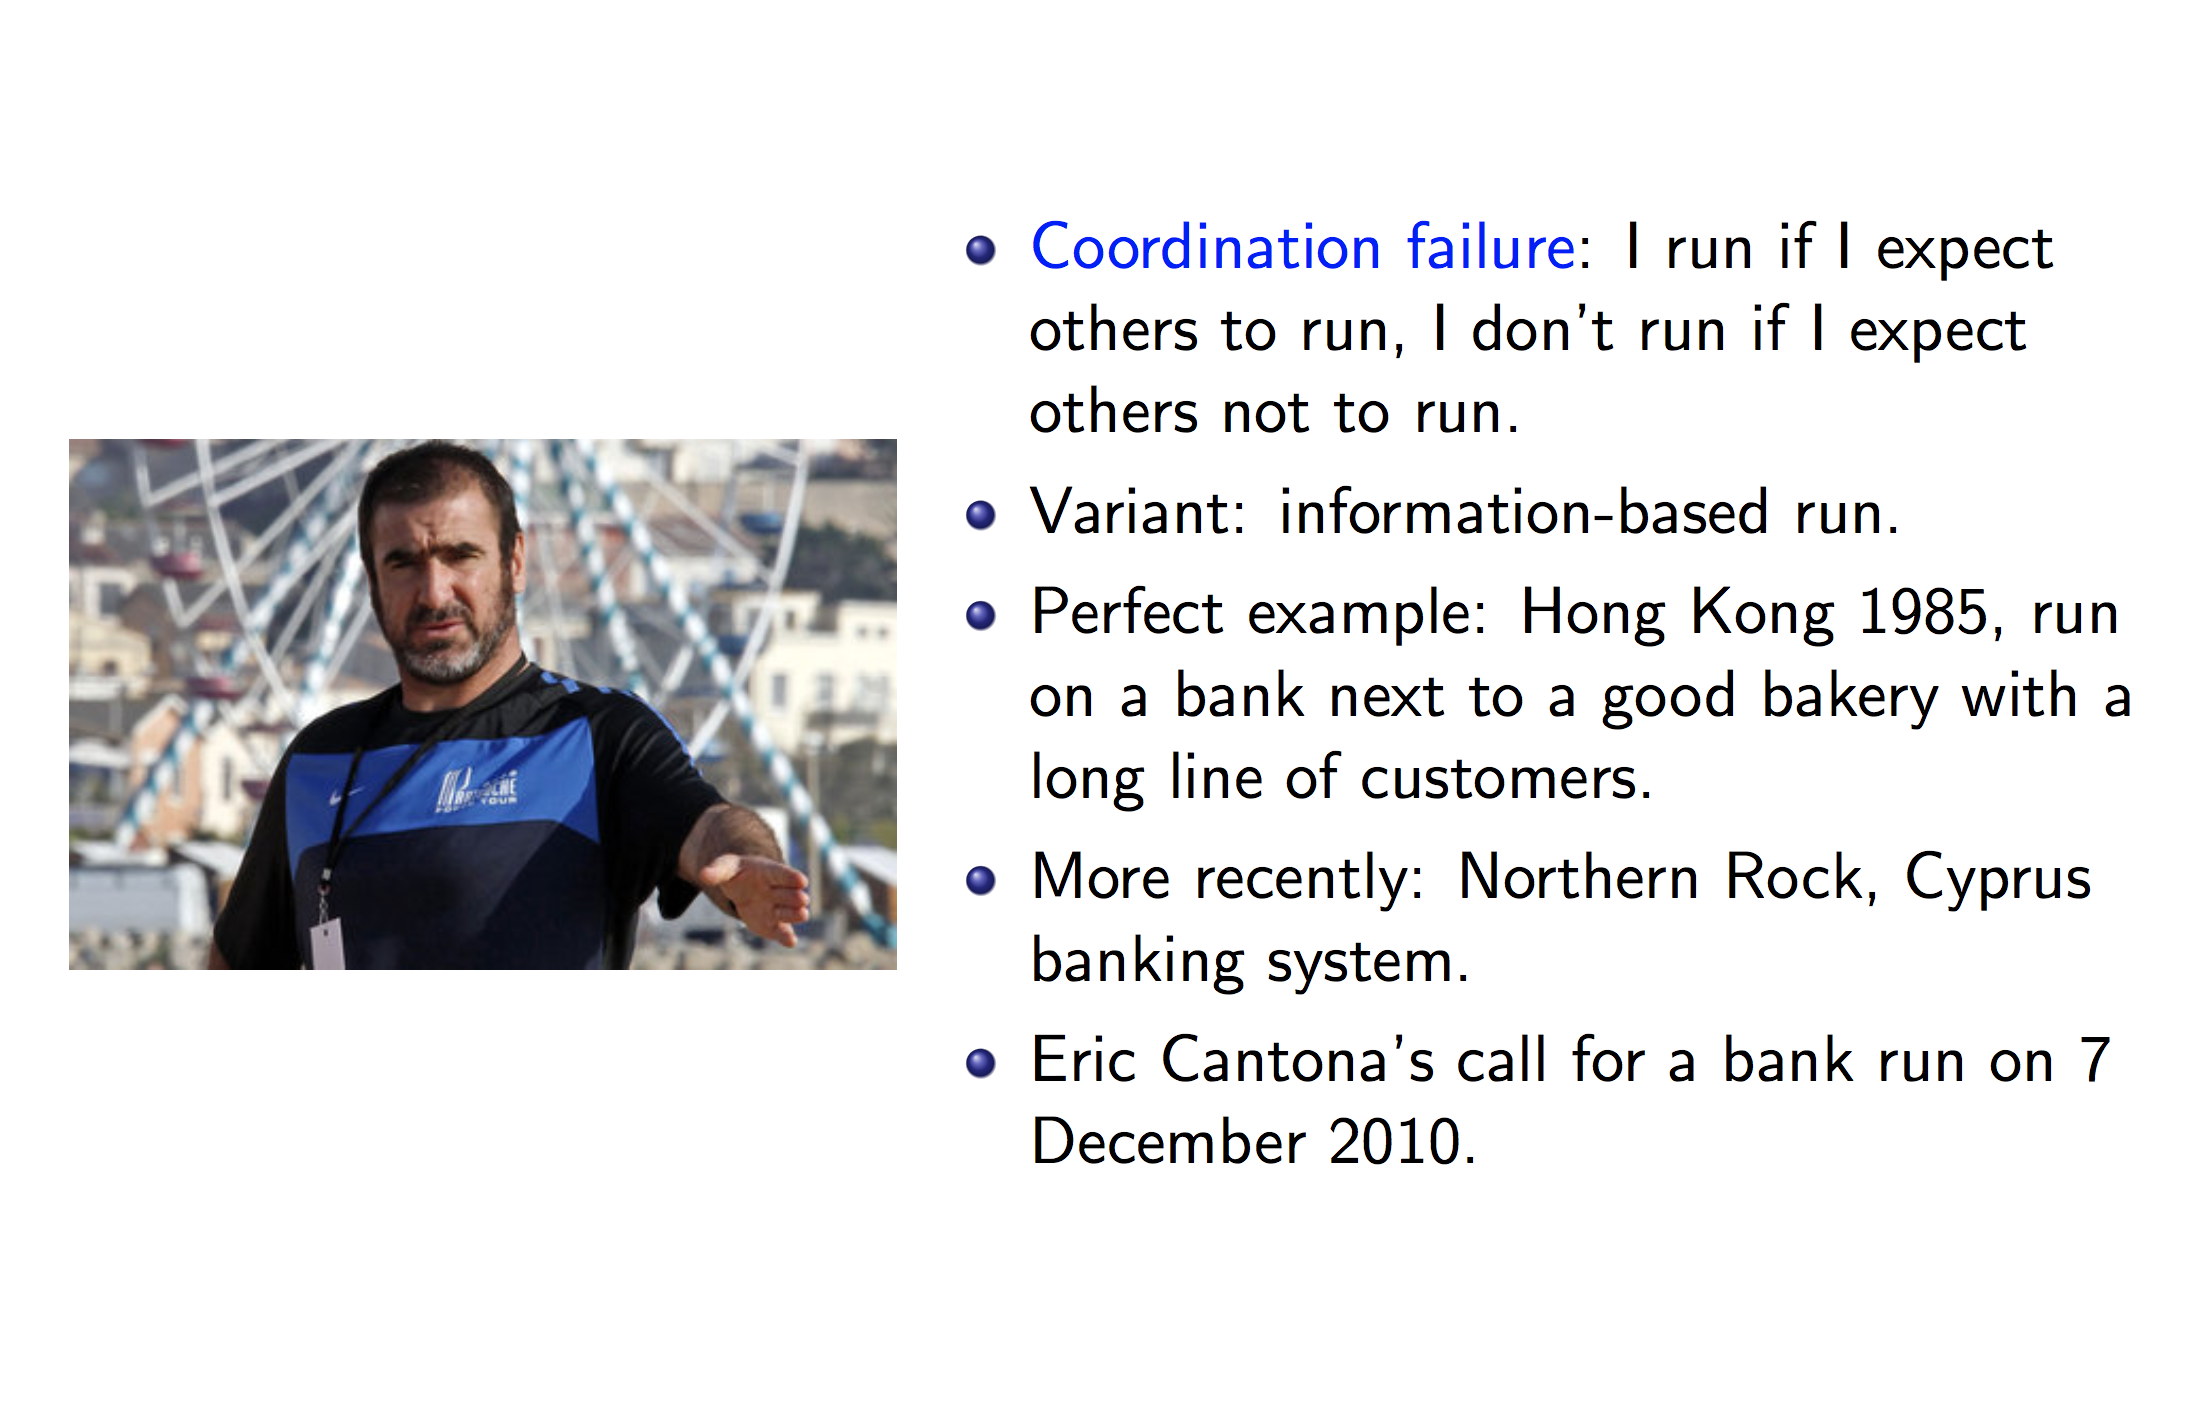
\includegraphics[width=\textwidth]{Figures/bank_runs3.png}
  \end{center}
\end{frame}




%======================================================================
\begin{frame}
  \begin{center}
    {\Large \textbf{A short history of banking and banking crises}}
  \end{center}
\end{frame}

\begin{frame}
\frametitle{US banks}
\begin{itemize}
\item No American banks as late as 1781
\item Alexander Hamilton writes to Congress’s superintendent of finance, Robert Morris, that \textit { “Most commercial nations have found it necessary to institute banks and they have proved to be the happiest engines that ever were invented for advancing trade.” }. Hamilton recommended that a bank be founded.
\item Morris persuaded Congress to charter the new nation’s first bank, \textit{the Bank of North America} located in Philadelphia in 1782.
\item Three years later, Boston merchants founded the Massachusetts Bank and Hamilton became a founder of the Bank of New York.
\item The irony: establishment of the \textit{First Bank of the United States} in 1791

\end{itemize}

\end{frame}

%---------------------------------------------------------------
\begin{frame}
\frametitle{US banks ... continued}
\begin{itemize}
\item First Bank of the United States was opposed for being unconstitutional
\item many fearing that it relegated undue powers to the federal government $\Rightarrow$ its charter was not renewed in 1811
\item War of 1812 $\Rightarrow$ government turning to state banks for finance... followed by over-expansion of credit
\item financial order needed to be reinstated
\item obtaining an official legislative charter was highly political



\end{itemize}
\end{frame}

\begin{frame}
\frametitle {Era of free banking}
\begin{itemize}
\item A new era of “free banking” emerged with a number of states passing laws in 1837 that abolished the requirement to obtain an officially legislated charter to operate a bank, and by 1860, a majority of states had issued such laws.
\item Anyone could operate a bank, one of the conditions was that all notes issued were back by proper security
\item still it did not guarantee immediate redemption in specie (gold or silver)
\item era of free banking suffered from financial instability with several banking crises occurring
\item  a disorderly currency characterized by thousands of different bank notes circulating at varying discount rates


\end{itemize}
$\Rightarrow$ The free banking era - characterized as it was by a complete lack of federal control and regulation - came to an end with the National Banking Act of 1863

\end{frame}

\begin{frame}
\begin{itemize}
\item National Banking Act of 1863 aimed to replace the old state banks with nationally chartered ones.
\item Office of the Comptroller of the Currency (OCC) was created to issue these new bank charters as well oversee that national banks maintained the requirement to back all note issuance with holdings of US government securities
\item new national banking system helped return the country to a more uniform and secure currency
\item growing complexity of the U.S. economy highlighted the inadequacy of an inelastic currency
\item frequent financial panics occurring throughout the rest of the nineteenth century
\item occurrence of the bank panic of 1907, it had become apparent that America’s banking system was out of date





\end{itemize}
\end{frame}


%----------------------------------------------------------------
\begin{frame}
\frametitle{Establishing the US Fed}

\begin{itemize}
\item  Congress created a new central bank, the Federal Reserve System (Fed) in 1913, after three-quarters of a century without a central bank - a period punctuated by a number of banking crises.
\item by end 1914 the twelve regional Reserve Banks, coordinated by the Federal Reserve Board in Washington, DC, were open for business.
\end{itemize}
\begin{figure}
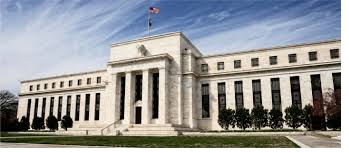
\includegraphics[]{Figures/Fed.png}
\end{figure}
\end{frame}

%--------------------------------------------------------------------

\begin{frame}
\frametitle{Background to US regulatory changes -\\ Leading up to 1929}
\begin{itemize}
  \item Separation of activities in banking came only after crash of 1929
\item Roaring Twenties
	\begin{itemize}
	\item Unprecedented economic boom in the US
    \item Mass production in manufacturing, telecommunication, movie and chemical sectors
    \item Population moved into cities to acquire jobs in these industries
    \item Americans - cash flush - invest in the stock market and deposit into banks
    \item Banks were opening at a rate of 4-5 per day (!)
	\end{itemize}

\end{itemize}

\end{frame}
%-----------------------------------------------------------------
\begin{frame}
\begin{figure}
	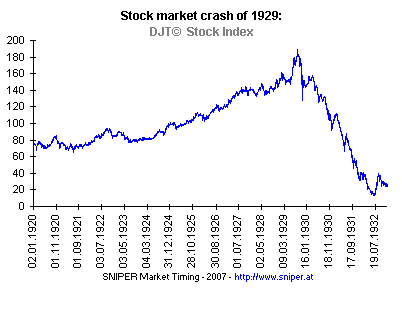
\includegraphics[width=1\textwidth]{Figures/Stockmarket.png}
\end{figure}

\end{frame}
%-------------------------------------------------------------------

\begin{frame}
\frametitle{Background to US regulatory changes - \\ The Great Depression (1929 - 1941)}
\begin{itemize}
\item 1929 stock market crash
	\begin{itemize}
	\item Stock market peaked on 3 Sept 1929
	\item 29 October 1929 - 40 per cent down. $\rightarrow$ Black Tuesday. Investors lost 14 billion dollars in a single day.
	\end{itemize}
\item Banks
\begin{itemize}
\item Banks lent money to investors to buy stock
\item Margin requirements were low
\item Banks were allowed to speculate and buy stocks for themselves
\item $\rightarrow$ The crash put a lot of pressure on banks
\end{itemize}
\end{itemize}


\end{frame}
%----------------------------------------------------------------------


\begin{frame}
\frametitle{Background to US regulatory changes - \\ The Great Depression (1929 - 1941)}
Once the selling began, more selling was needed to satisfy margin calls and liquidity requirements for banks....
\\

\begin{itemize}
\item Bank runs
\begin{itemize}
\item No guarantees on cash at the bank
\item People feared that their bank would collapse
\item Some banks were not able to fulfill the requests for withdrawal and closed their doors to people
\item $\downarrow$ lending to businesses and consumers
\item $\rightarrow$ more people need to withdraw money
\item paper money was backed by gold
\item people kept money under their mattresses
\end{itemize}

\end{itemize}

\end{frame}
%------------------------------------------------------------------
\begin{frame}
\begin{figure}
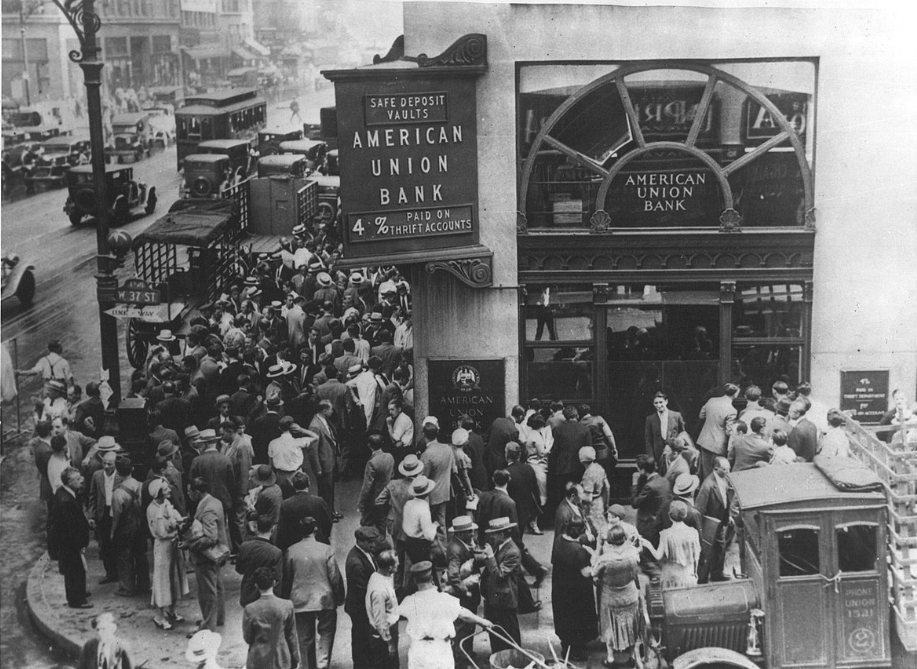
\includegraphics[width=1\textwidth]{Figures/Bankrun.png}
\end{figure}
\end{frame}



%-------------------------------------------------------------------
\begin{frame}
\frametitle{The US Federal Reserve and the Great Depression}

\begin{itemize}
\item The government began to increase interest rates, in 1929, from 3.5$\%$ to 5$\%$.
\item Money supply not stabilised - supply fell by 30$\%$ between 1929 and 1933
\item prices dropped
\item banks failed
\item $\Rightarrow$ deflation
\item $\Rightarrow$ No confidence in banking sector
\item Focus was on maintaining the gold standard - sufficient gold reserves to meet the demands of the depositor, and adequate demand for currency

\end{itemize}


\end{frame}

%---------------------------------------------------
\begin{frame}
\frametitle{Great Depression Effects on the Economy}
\begin{itemize}
\item \textbf{Higher unemployment} By 1933, the unemployment rate had climbed from 3$\%$ to 25$\%$
\item \textbf{Lower income} On average incomes were reduced by 40 $\%$
\item \textbf{Deflation}
\item \textbf{Increased foreclosures} By 1934, nearly one-half of all residential loans were delinquent and over 1 million families lost their farms
\item \textbf{Banks close} In 1933 alone, more than 4 000 banks closed
\item \textbf{Hollywood} actually did very well during this period of time - the Hollywood film industry. It is thought that people went to the movies because, for a brief time while at the movie, they could forget their many hardships :)

\end{itemize}
\end{frame}

%-------------------------------------------------------------------
\begin{frame}
\frametitle{Bank Holiday of 1933}
An effort to stem bank failures and ultimately restore confidence in the financial system
\begin{itemize}
\item 36 hours after taking office in March 1933, President Roosevelt ordered the suspension of all banking transactions, effective immediately
\item For an entire week, Americans would have no access to banks or banking services.
\item Before banks could reopen, there needed to be agreement on whether or not to “weaken the link between gold and note issue” (Meltzer 2003, 423)
\item The crisis began to subside on 9 March, when Congress passed the Emergency Banking Act.
\item On March 13, member banks in Federal Reserve cities received permission to reopen.
\item By March 15, banks controlling 90$\%$ percent of the country’s banking resources had resumed operations and deposits far exceeded withdrawals.... the worst of the banking crisis seemed to be over.
\end{itemize}
\end{frame}




%---------------------------------------------------------------------

\begin{frame}
\frametitle{Policy changes during the great depression}

Role of the US Government changed dramatically

\begin{itemize}
\item Banking Act of 1933
\begin{itemize}
\item Glass-Stegall Act - breaks connection between commercial and investment banks
\item Federal Deposit Insurance Corporation (FDIC) - insure bank deposits
\item Regulation Q - outlawed the payment of interest on checking accounts and also placed ceilings on the amount of interest that could be paid on other deposits
\end{itemize}

\item 1933: The US goes off the gold standard
\item 1934: Securities and Exchange Act - helped to police activities related to the selling of securities
\item 1935: Social Security Act - assistance to the unemployed, handicapped and elderly
\item  Banking Act of 1935 - fully insured balances up to $\$$5,000 and provided no insurance for balances above that amount
\end{itemize}
\end{frame}

% \begin{frame}
% \begin{figure}
% \frametitle{President Franklin D. Roosevelt signs the Glass-Steagall banking bill in 1933}
% 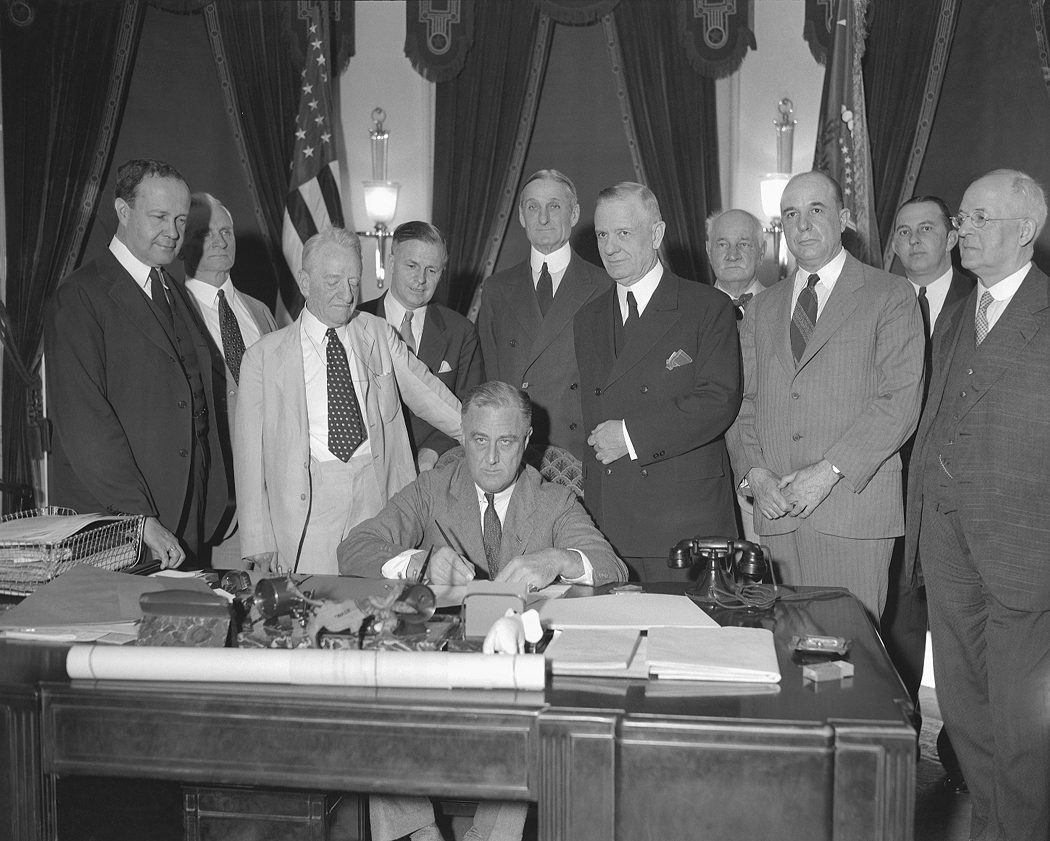
\includegraphics[width=1\textwidth]{Figures/GS1.png}
% \end{figure}
% \end{frame}

%--------------------------------------------------------------------
\begin{frame}
\frametitle{Glass-Steagall recap}
Over time, the term Glass–Steagall Act came to be used most often to refer to four provisions of the 1933 Banking Act that separated commercial banking from investment banking.\\
\begin{itemize}
\item Glass-Steagall Act is a law that prevented banks from using depositors' funds for risky investments (stock market) \\$\Rightarrow$ Separated investment banking from retail banking
\item Institutions were given one year to decide whether they wanted to specialize in commercial or investment banking.
% \item Glass-Steagall was enacted as an emergency response
\end{itemize}
\end{frame}

%---------------------------------------------------------------------
\begin{frame}
\frametitle{Justification of the rate ceilings - Regulation Q}
\begin{itemize}
\item Shield bank profits by limiting the competition for
deposits: competition for deposits not only reduced bank profits by raising interest expenses, but also could cause banks to seek riskier investments and make high risk loans in order to cover the costs.
\item Encourage country banks to lend more in their local communities rather than hold balances with larger banks in financial centers.
\item {Deposit interest rate ceiling would compensate banks for the costs incurred by the newly introduced
deposit insurance premiums}
\item {Ceilings were extended to thrift institutions} such as
mutual savings banks, savings and loan associations in 1966 - policymakers believed that competition for deposits between commercial banks and thrifts as one of the reasons of the rise in residential mortgage interest rates and the subsequent slowdown in lending growth

\end{itemize}
\end{frame}

\begin{frame}
\frametitle{Issues with Glass-Steagall}

\begin{itemize}
\item Limiting deposit interest rate competition through rate limitations
\item Restricting competition for deposits based on financial strength by insuring depositors
\item Critics argued that Regulation Q's limits on interest rates created the "disintermediation" that began in the 1960s
\item Allowed commercial banks to earn high profits until nonbanking companies found ways to offer substitutes for bank loans and deposits...
\item ... Over time, Regulation Q made bank deposits less attractive relative to other savings products and helped boost fund industry growth,
particularly, money market mutual funds.
\item $\Rightarrow$ the development of substitutes to bank deposits
\end{itemize}
\end{frame}

%----------------------------------------------------------------

\begin{frame}
\begin{figure}
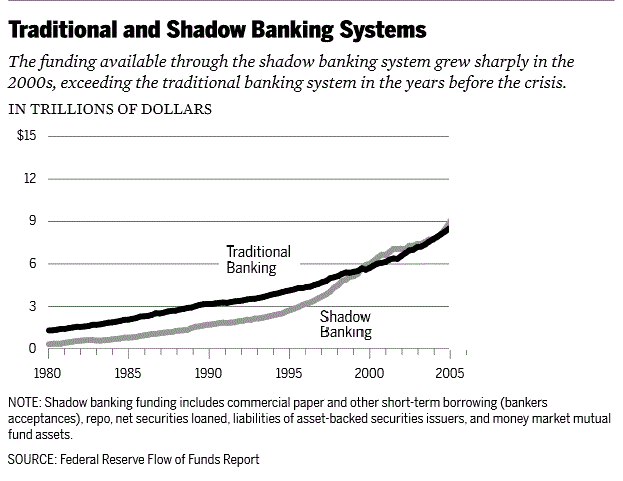
\includegraphics[width=1 \textwidth]{Figures/SB1.png}
\end{figure}
\end{frame}

%----------------------------------------------------------------

\begin{frame}
\frametitle{Federal guarantees in the mortgage market}
The rise of securitization, in the 1980s, was strongly supported by the introduction of federal guarantees in the mortgage market
\begin{itemize}
\item The US housing policy and particularly the introduction of
federal guarantees in mortgages markets helped transform
the funding structure of the US economy
\item The creation of GSEs planted the seeds for linking mortgage markets with broader capital markets...
\item by creating a strong secondary mortgage market for housing loans in order to  provide a stable source of funding for residential mortgages across the country (particularly for low- and moderate-income households)
\item  ‘originate to distribute’ model
\end{itemize}
\end{frame}

%--------------------------------------------------------------------

\begin{frame}
\begin{figure}
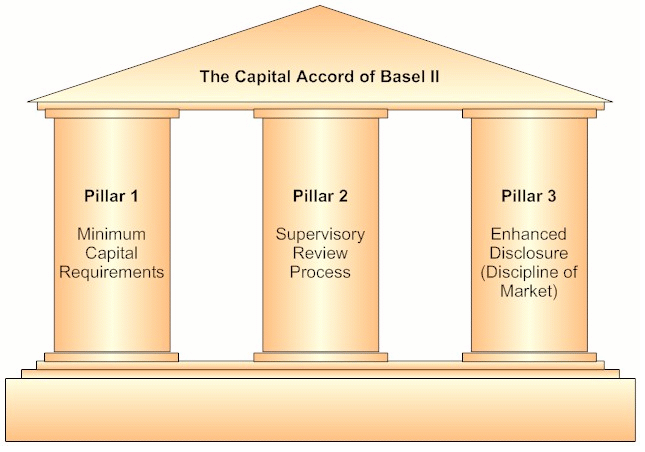
\includegraphics[width=1 \textwidth]{Figures/BaselII.png}
\end{figure}
\tiny{Source: IBM}
\end{frame}

%--------------------------------------------------------------------

\begin{frame}
\begin{center}
  {\Large \textbf{The Global Financial Crisis}}
\end{center}
\end{frame}

%--------------------------------------------------------------------
\begin{frame}
  \begin{figure}
    \begin{center}
      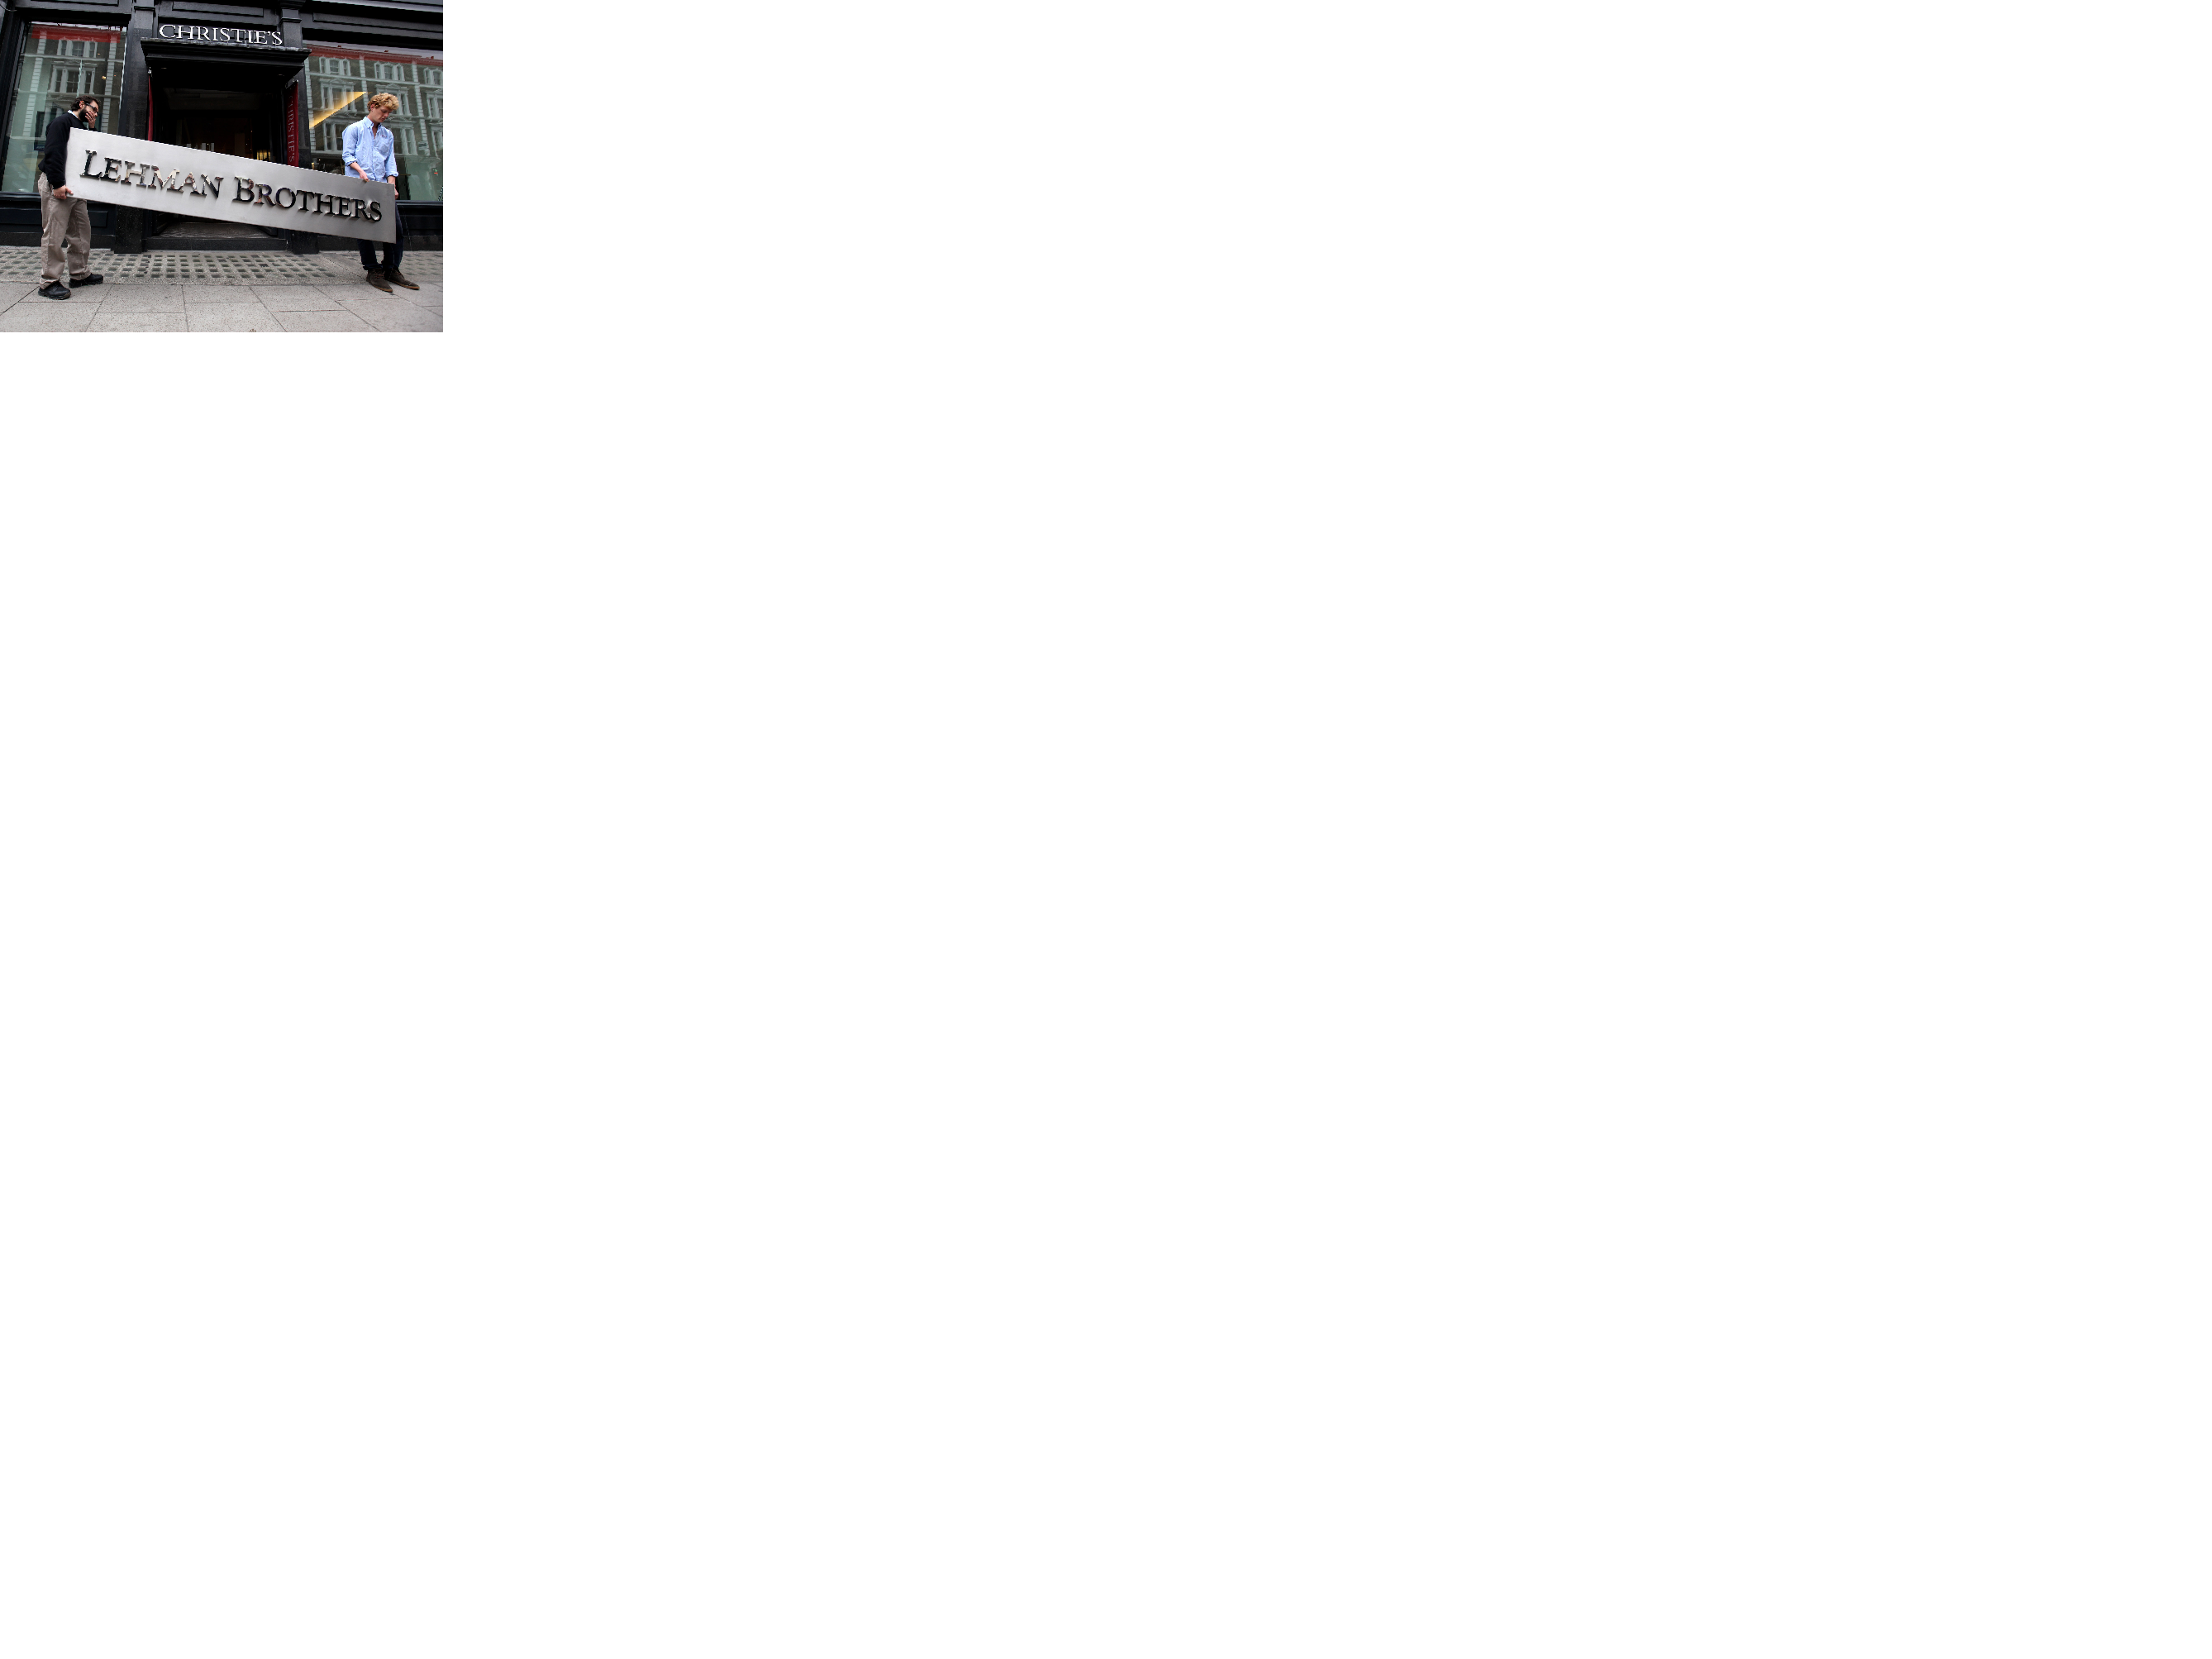
\includegraphics[width=5\textwidth]{Figures/Lehman.png}
    \end{center}
  \end{figure}
\end{frame}

\begin{frame}
\frametitle{Leading up to the crisis}
\begin{itemize}
\item Massive new inflows of capital into the US, mostly from oil-producing and Asian countries since the early 2000s
\item Increase in house prices in the US (also Spain,
Ireland, …)
\item Mid-2006: house prices begin to stagnate
\item February 2007: Prices of Credit Default Swaps for sub-prime
mortgages in the US collapse by 30 $\%$.
\item Mid-June 2007: Bear Stearns injects $\$$3.2 billion in two hedge funds in order to avoid their liquidation.
\item End July 2007: American Home Mortgage Investment Corp. ceases
interest payments, bankruptcy on 6 August.
\item 9 August: BNP Paribas suspends payouts for 3 investment funds
because of the impossibility to value underlying assets.
\end{itemize}
\tiny{Source: E von Thadden 2012}
\end{frame}


%---------------------------------------------------------------
\begin{frame}
\begin{itemize}
\item September – December: increasing write-downs on
mortgage backed securities
\item January 2008: Hypo Real Estate (Germany) acknowledges
temporary funding problems
\item March 5: Carlyle Capital (NY) bankrupt. Bear Stearns suffers major losses.
\item March 13: Bear Stearns obtains no more funding on the repo market
\item March 14-16: Federal Reserve Bank of New York brokers the acquisition of Bear Stearns by JP Morgan Chase for $\$$236 million, loan of $\$$30 billion to JP Morgan Chase.
\item September 15: Lehmann Brothers bankrupt with $\$$613 billion of debt, Merrill Lynch taken over by Bank of America.
\end{itemize}
\tiny{Source: E von Thadden 2012}
\end{frame}

%---------------------------------------------------------------

\begin{frame}
\begin{figure}
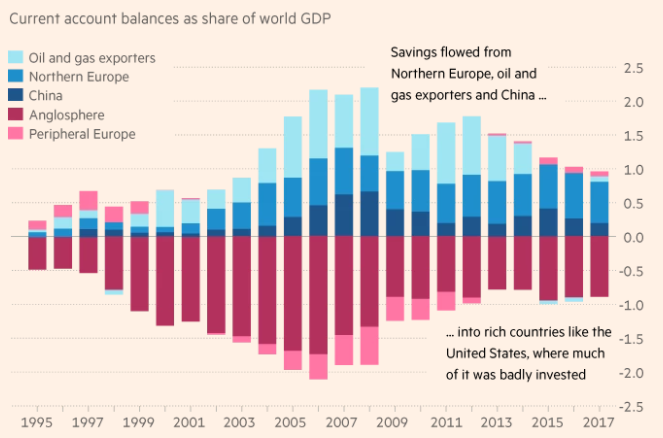
\includegraphics[width=1\textwidth]{Figures/SavingsGlut.png}
\end{figure}
\tiny{Source: Financial Times. https://www.ft.com/content/56d25a52-7df5-11e7-9108-edda0bcbc928}
\end{frame}
%---------------------------------------------------------------

\begin{frame}
\begin{figure}
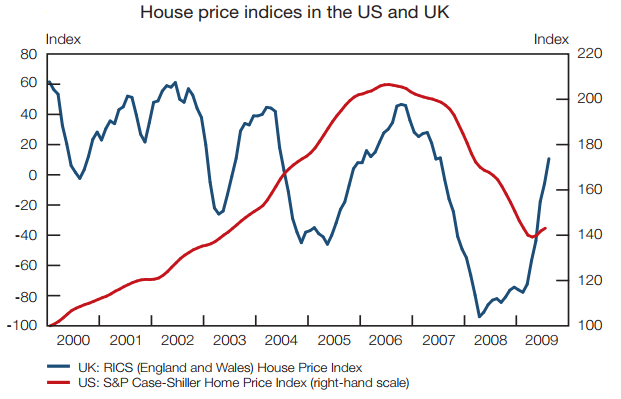
\includegraphics[width=1\textwidth]{Figures/HPUS.png}
\end{figure}
\tiny{Source: Financial Stability Review, Sept 2009, SARB}
\end{frame}


\begin{frame}
\begin{figure}
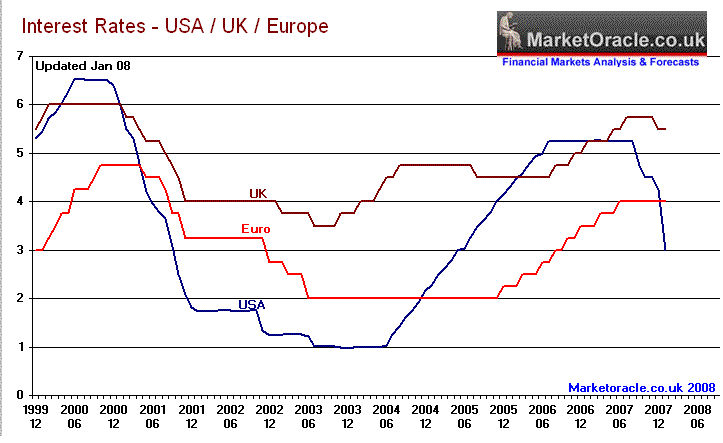
\includegraphics[width=1\textwidth]{Figures/Intrate.png}
\end{figure}
\tiny{Source: Market Oracle.co.uk}
\end{frame}

\begin{frame}
\frametitle{NINJA loans}
\begin{figure}

\includegraphics[width=1 \textwidth]{Figures/Ninja.png}
\end{figure}
Generally lenders require the borrower to show a stable stream of income or sufficient collateral. A NINJA loan ignores the verification process

\end{frame}

\begin{frame}
\frametitle{NINJA = No Income, No Job or Assets}
\begin{itemize}
\item Sub-prime mortgages were mis-sold in their millions by lenders desperate to feed the pipeline for securitising, or packaging up, these loans by investment banks
\item Research by the industry's regulator, the Financial Services Authority:
\begin{itemize}
\item Poor practices by mortgage brokers (account for more than 60 per cent of all mortgages sold) and lenders
\item In half the cases it investigated customers had self-certified their income
\item Significant numbers of consumers' had been advised to remortgage - thus incur additional charges, without the adviser being able to demonstrate that this was beneficial to the customer
\item In a third of cases the intermediaries failed to assess properly the borrower's ability to afford the mortgages
\item Lenders had inadequate lending standards which they often failed to apply properly
\end{itemize}
\end{itemize}
\end{frame}

%------------------------------------------------------------

\begin{frame}
\frametitle{More on the Causes of the Crisis}
\begin{itemize}
\item Excessive US mortgage lending
\item Excessive securitization
\item Failure of bank risk models
\item Inadequate corporate governance of banks
\item Faulty financial regulation: - systemic risk, shadow banking?
\item Systemically Important Financial Intermediaries
\item Break-down of interbank market
\item Biased rating agencies
\item Savings glut (China, Middle East, Germany, …)
\item Real-estate price bubble (US, UK, Spain, …)
\item US Federal Reserve interest rate policy
\end{itemize}
\tiny{Source: E von Thadden 2012}
\end{frame}

\begin{frame}
  \frametitle{Write-downs of Large US Institutions}
\begin{figure}
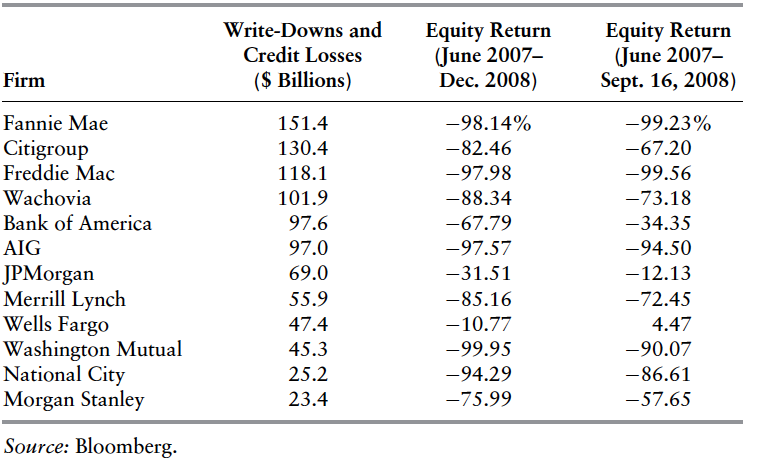
\includegraphics[width=\textwidth]{Figures/table6_1.png}
\end{figure}
\end{frame}

\begin{frame}
\end{frame}

%------------------------------------------------------------

\begin{frame}
  \frametitle{Regulatory Arbitrage - How it Works}
  \begin{center}
    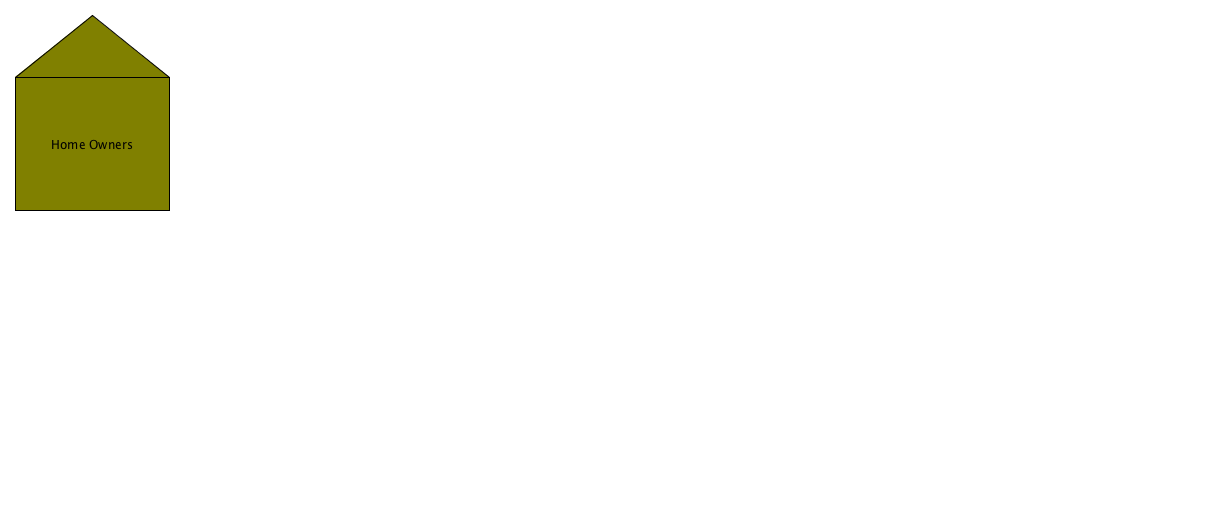
\includegraphics[width=\textwidth]{Figures/Securitization1.png}
  \end{center}
\end{frame}
\begin{frame}
  \frametitle{Regulatory Arbitrage - How it Works}
  \begin{center}
    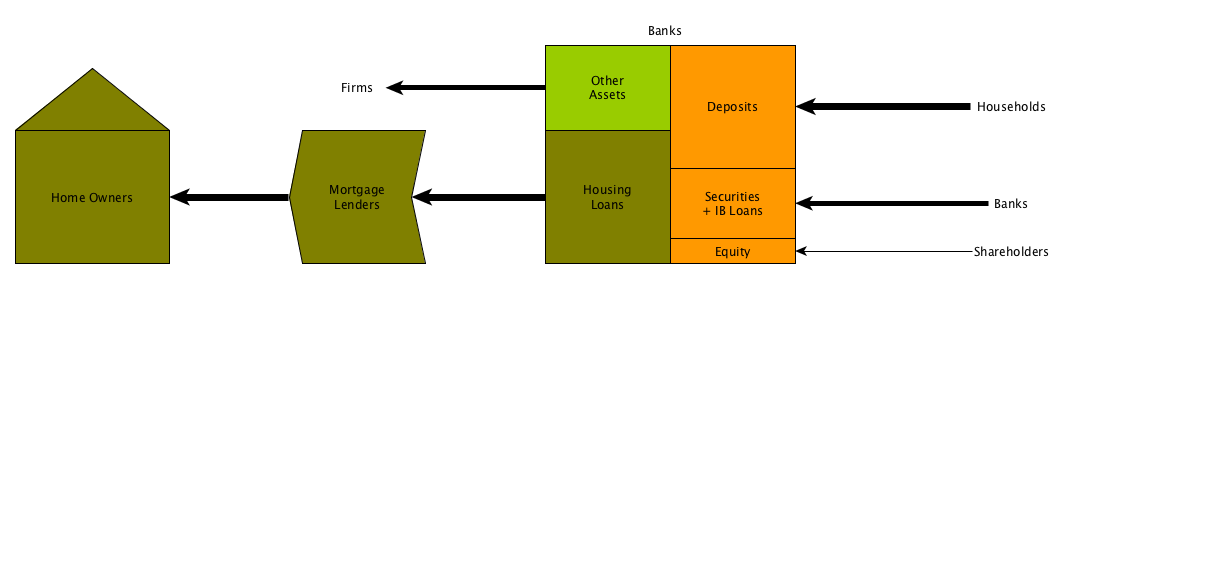
\includegraphics[width=\textwidth]{Figures/Securitization2.png}
  \end{center}
\end{frame}
\begin{frame}
  \frametitle{Regulatory Arbitrage - How it Works}
  \begin{center}
    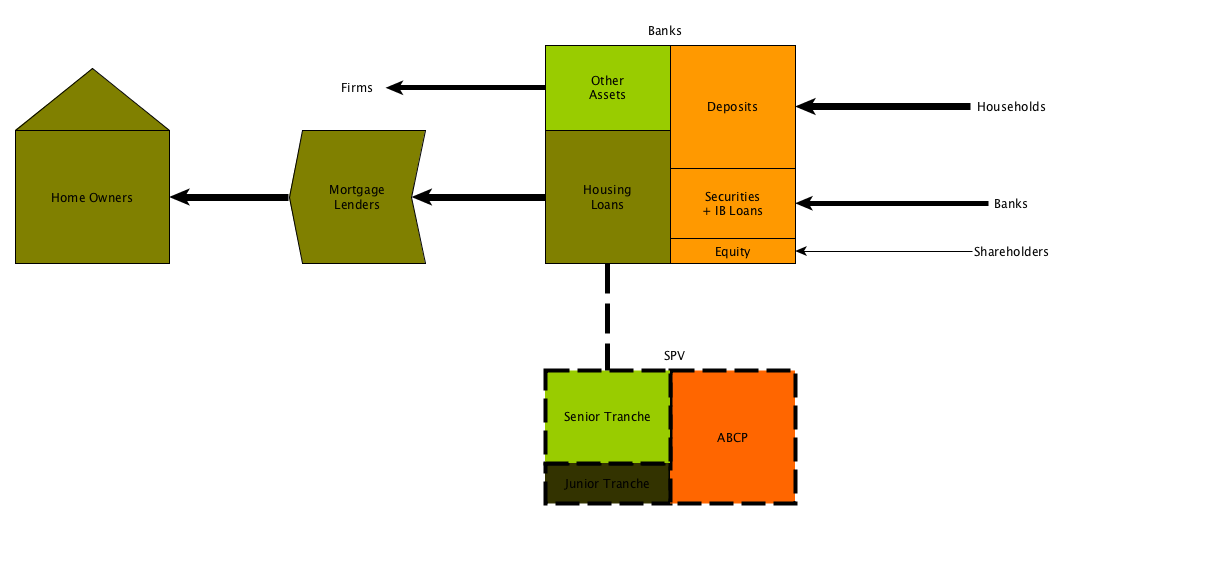
\includegraphics[width=\textwidth]{Figures/Securitization3.png}
  \end{center}
\end{frame}
\begin{frame}
  \frametitle{Regulatory Arbitrage - How it Works}
  \begin{center}
    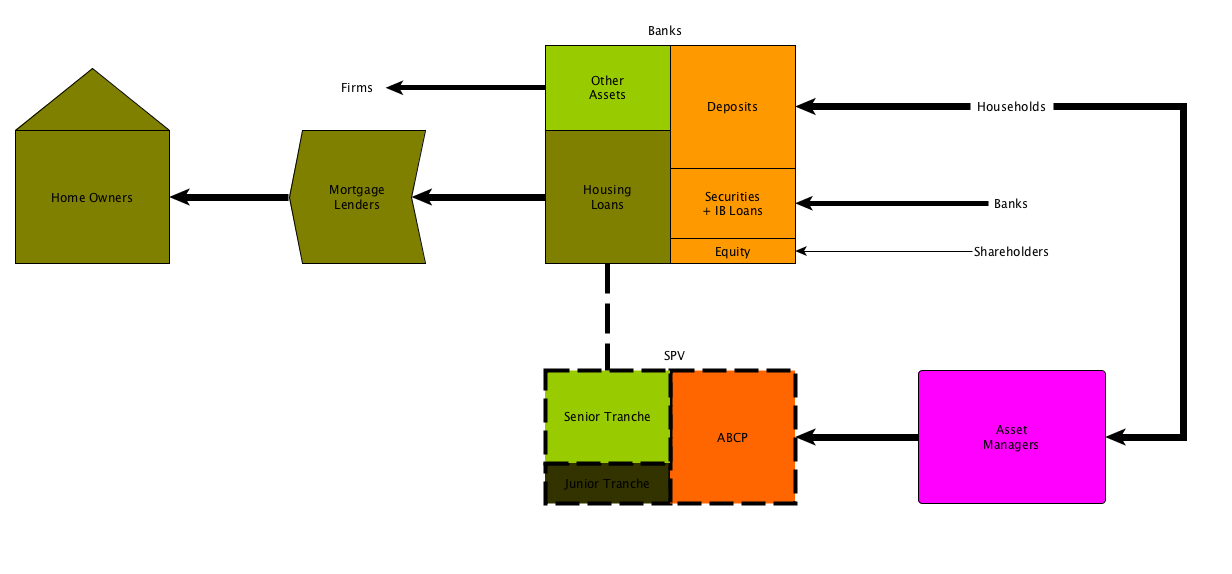
\includegraphics[width=\textwidth]{Figures/Securitization4.png}
  \end{center}
\end{frame}

%------------------------------------------------------------

\begin{frame}
Financial Crisis timeline
\begin{figure}
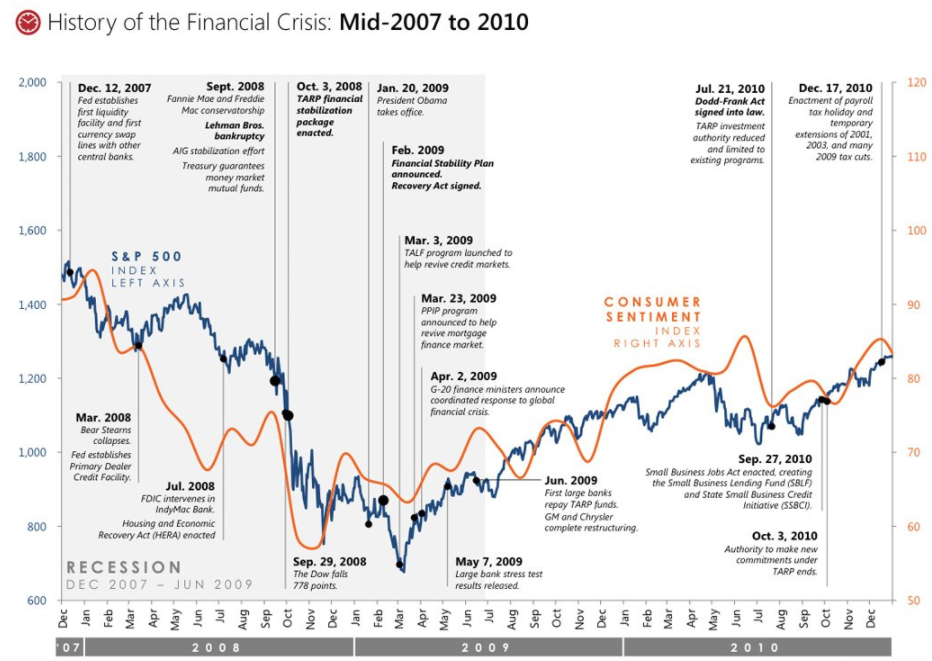
\includegraphics[width=1\textwidth]{Figures/GFC1.png}
\end{figure}
\tiny{Source:http://www.businessinsider.com/chart-financial-crisis-2013-9}
\end{frame}

\begin{frame}
\begin{center}
\centering{\Large Introduction to shadow banking}
\end{center}
\end{frame}

\begin{frame}
\frametitle{Shadow banking - history}
\begin{itemize}
\item \textit{Shadow banking} coined in 2007
\item Prior to 2007 - known as market-based finance or non-banks
\item A lot of focus on developments in the US
\item US Money-market mutual funds: 1970
\item US Cash management accounts: 1977
\item Less-regulated market for capital grew rapidly next to the traditional banking system
\item Regulatory arbitrage
$\rightarrow$ Deregulation
\end{itemize}
\end{frame}

\begin{frame}
\frametitle{Why worry about shadow banking?}
\begin{itemize}
\item Systemic risk
\item Regulatory arbitrage
\item Monetary policy transmission
\item Channel for capital flows
\item Financial inclusion
\end{itemize}
\end{frame}

\begin{frame}
\frametitle{Distribution of financial assets globally}
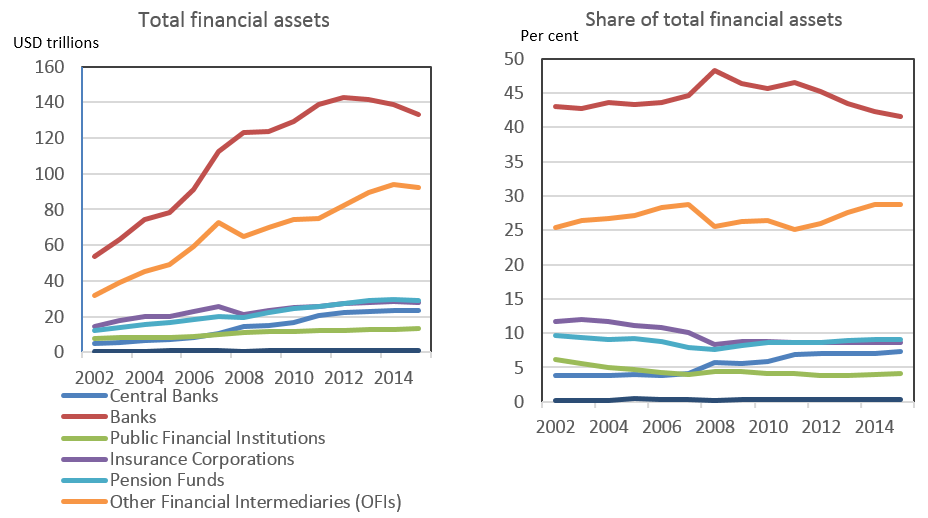
\includegraphics[width=\textwidth]{Figures/shadowbank5.png}
\end{frame}

\begin{frame}
\frametitle{Distribution of financial assets among FIs in South Africa}
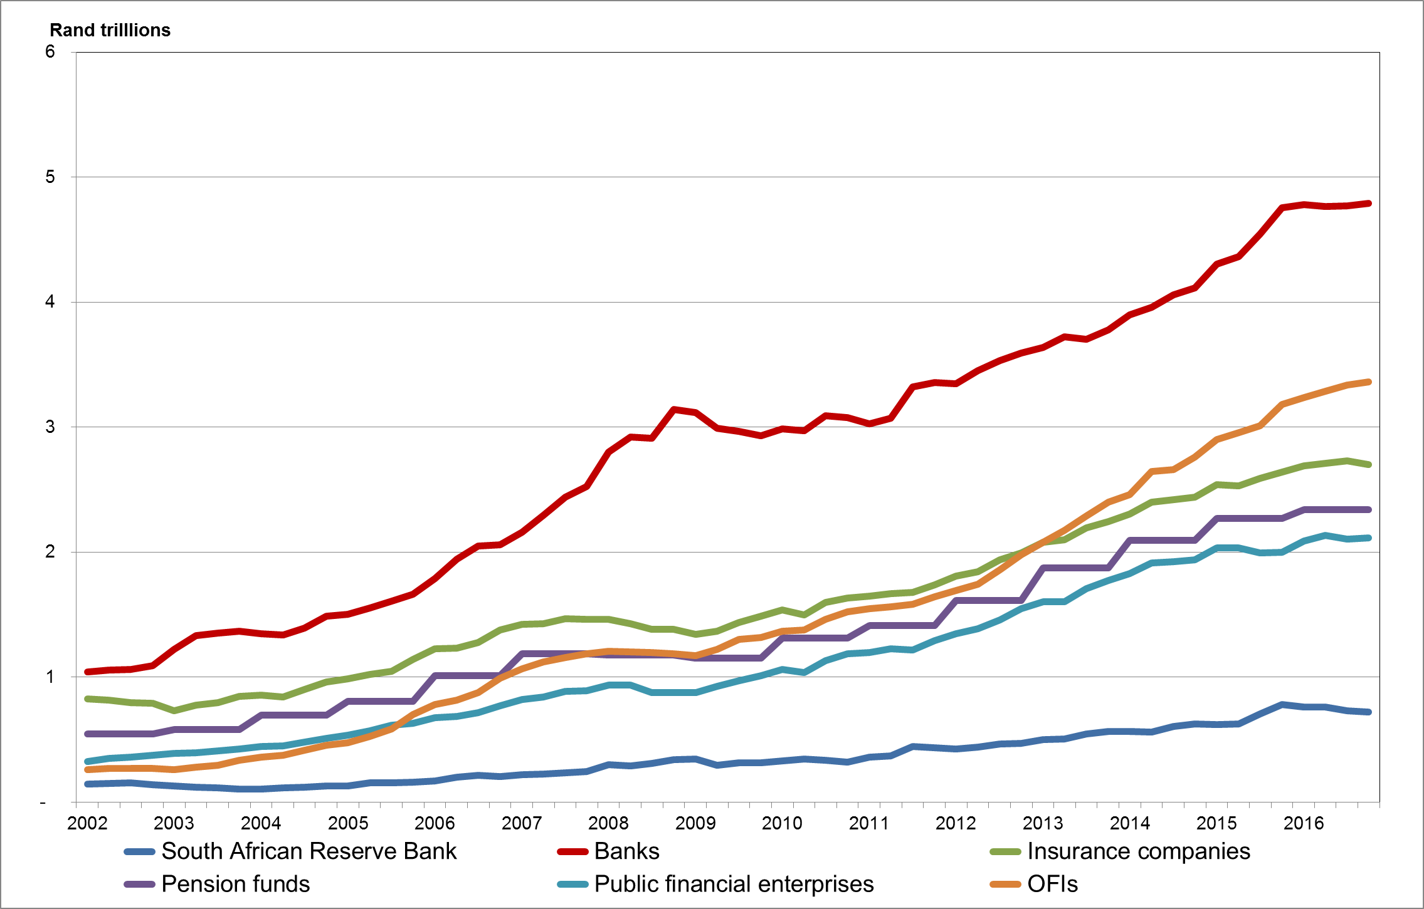
\includegraphics[width=\textwidth]{Figures/shadowbank7.png}
\end{frame}

\begin{frame}
  \begin{center}
    {\Large \textbf{A Quick Overview of Monetary Policy}}
  \end{center}
\end{frame}

\begin{frame}
\frametitle{The Balance Sheet of the Federal Reserve}
\begin{center}
  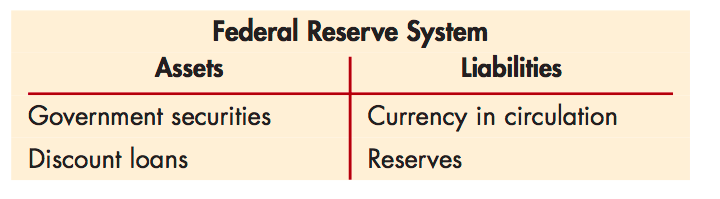
\includegraphics[width=0.8\textwidth]{Figures/FedBS1.png}
\end{center}
\begin{itemize}
  \item Currency in circulation are IOUs backed by legal promise to be repaid
  \item All banks have to hold required reserves (2\% of deposits) and hold excess reserves at Fed
  \item Assets are mostly government securities obtained in open market operations
\end{itemize}
\end{frame}

\begin{frame}
\frametitle{Central Bank Operations}
Open Market Operations
\begin{center}
  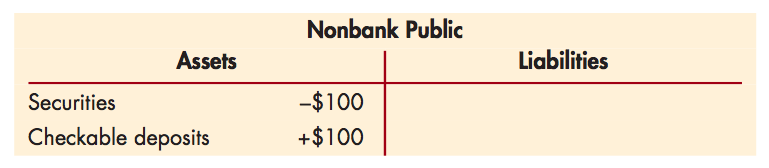
\includegraphics[width=0.8\textwidth]{Figures/OMO1.png}\\
  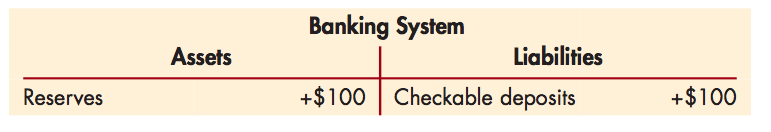
\includegraphics[width=0.8\textwidth]{Figures/OMO2.png}\\
  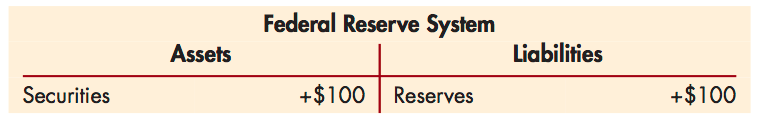
\includegraphics[width=0.8\textwidth]{Figures/OMO3.png}
\end{center}
Discount Lending:
\begin{center}
  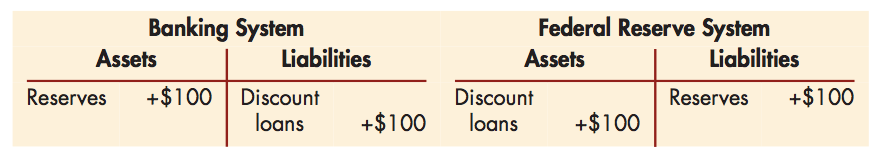
\includegraphics[width=0.8\textwidth]{Figures/DiscountLending1.png}\\
\end{center}
\end{frame}

% -----------------------------------------------------------------------------
\begin{frame}
\frametitle{Some final thoughts continued}
\begin{itemize}
\item If the ultimate purpose of regulation is to protect the consumer and serve systemic interests, then it should be subjected to the test of whether it does so effectively and cost-efficiently
\item arguments against particular mechanisms may not invalidate the arguments for regulation in general
\item the rationale for all regulatory arrangements and structures needs to be clearly identified rather than taken for granted
\item Therefore regulation should be an evolving process, responsive to changes in the market environment
\item Regulation that remains stable irrespective of market changes will be inefficient at best, and perhaps even perverse.
\end{itemize}
% \tiny{Source: Financial Regulation in South Africa, Falkena \textit{et al}, 2001}
~\\
~\\
~\hfill \mcdbl{Thank you!}
\end{frame}
\end{document}
